%\begin{tcolorbox}[breakable,colback=black!5!white,colframe=red!80!black,width=\textwidth]
%%\begin{tcolorbox}[breakable,colback=black,colframe=black,width=\textwidth]
\chapter{Theoretical motivation}
%\end{tcolorbox}
\label{chap:theory}

The standard model (SM) represents, so far, the best available description of the elementary particles and their interactions. It is the summation of two gauge theories: the electroweak interaction, that portrays the weak and electromagnetic interactions together, and the strong interaction, or quantum chromodynamics (QCD). Particles, namely quarks and leptons, are described as spin-1/2 fermions, whilst interactions are mediated by spin-1 bosons. The symmetry group of the standard model is:

\begin{equation}
SU_{C}(3) \times SU_L (2) \times U_Y (1),
\label{eq:theory_SMgroup}
\end{equation}

\noindent where the first factor is related to strong interaction, whose mediators are eight gluons, while $SU_L (2) \times U_Y (1)$ is the electroweak symmetry group, whose mediators are the photon and the $Z$-$W^{\pm}$ bosons.\\
In renormalizable theories, with no anomalies, all gauge bosons are expected to be massless, in contrast with our experimental knowledge. This inconsistency is solved by introducing a new scalar particle, the Higgs boson, that gives mass to weak bosons and fermions via the spontaneous symmetry breaking mechanism.
\\

\noindent In the last decades, the standard model has been accurately probed by many experimental facilities (LEP, Tevatron, LHC), and the results lead to an impressive agreement between theoretical predictions and experiments~\cite{Baak:2013ppa}. The discovery of the Higgs boson at the CERN Large Hadron Collider, measured by both the CMS and the ATLAS Collaborations~\cite{bib:Aad20121,bib:Chatrchyan201230,bib:Chatrchyan2013lba,Aad:2013xqa,Khachatryan:2014jba,Aad:2014aba,Aad:2015zhl}, represents not only an extraordinary confirmation of the model, but also the latest biggest achievement in particle physics as a whole.

\section{Beyond standard model theories}
Even though the SM is the most complete picture of the universe of the particles, many questions are still left open. From a phenomenological point of view, some experimental observations are not included in the theory:
\begin{itemize}
\item in SM, neutrinos are massless (whilst the well established observation of neutrino flavour oscillation proves that neutrinos do carry mass);
\item no candidates for dark matter are predicted;
\item no one of the fields included in the SM can explain the cosmological inflation;
\item the CP asymmetry embedded in the SM is not sufficient to explain the matter-antimatter asymmetry in the universe.
\end{itemize}
From a purely theoretical perspective, some issues are still relevant in the formulation of the model:
\begin{itemize}
\item {\itshape Flavour problem.}\\ The standard model has 18 free parameters: 9 fermionic masses; 3 angular parameters in the Cabibbo-Kobayashi-Maskawa matrix, plus 1 phase parameter; electromagnetic coupling $\alpha$; strong coupling $\alpha_{\text{strong}}$;  weak coupling $\alpha_{\text{weak}}$; $Z$ mass; the mass of the Higgs boson. Such a huge number of degrees of freedom marks the SM as weakly predictive in the flavour sector.
\item {\itshape Unification.}\\ There is not a ``complete'' unification of strong, weak and electromagnetic interactions, since each one has its own coupling constant, behaving differently at different energy scales; not to mention the fact that gravitational interaction is completely excluded from the SM.
\item {\itshape Hierarchy problem.}\\ From quantum field theory, it is known that perturbative corrections to the mass of the scalar bosons included in the theory tend to make it increase towards the energy scale at which the considered theory still holds~\cite{Degrassi:2012ry}. If the standard model is seen as a low-mass approximation of a more general theory valid up to the Planck mass scale (\textit{i.e.},~$\sim~1.2~\times~10^{19}$~GeV), a fine-tuning cancellation of the order of $1$ over $10^{34}$ is needed to protect the Higgs boson mass at the electroweak scale ($\sim 100$ GeV). Such an astonishing correction is perceived as very unnatural.
\end{itemize}

\noindent Numerous beyond standard model theories (BSM) have been proposed in order to overcome the limits of the SM.\\
Grand Unified Theories (GUT) aim at extending the symmetry group of the SM (eq.~\ref{eq:theory_SMgroup}) into largest candidates, such as $SO(10)$, $SU(5)$ and $E(6)$. At GUT scale, approximately at $10^{16}$ GeV, non-gravitational interactions are expected to be ruled by only one coupling constant, $\alpha_{GUT}$.\\%Pur godendo di alcuni punti di forza, quali la possibilit\`a di dare massa ai neutrini ammettendo l'esistenza del neutrino right alla scala GUT, queste teorie prevedono in alcuni casi fenomeni non ancora osservati (decadimento del protone, esistenza dei monopoli magnetici) e sono valide ad energie non riproducibili sperimentalmente. Qualche speranza di trovare nuova fisica a scale inferiori potrebbe nascere dal connubio tra GUT e modelli supersimmetrici.
Super symmetric (SUSY) models~\cite{Martin:1997ns} state that every fermion (boson) of the SM has a bosonic (fermionic) superpartner, with exactly the same quantum numbers, except the spin. If SUSY is not broken, each couple of partners and superpartners should have the same masses, hypothesis excluded by the non-observation of the s-electron. Super symmetry represents a very elegant solution of the hierarchy problem of the Higgs boson mass, since the perturbative corrections brought by the new SUSY particles exactly cancel out the divergences caused by the SM particles corrections. A particular sub-class of SUSY models, minimal super symmetric standard models~\cite{Csaki:1996ks,Castano:1993ri,Haber:1993wf}, is characterized by the introduction of a new symmetry, the R-parity, that guarantees the proton stability and also the stability of the lightest SUSY particle, a possible good candidate for dark matter.
\\

\noindent Two other possible theoretical pictures are extensively described in sec.~\ref{sec:theory_HVT}-\ref{sec:theory_WED}.

\newpage

\section{Heavy Vector Triplet}
\label{sec:theory_HVT}

The heavy vector triplet model~\cite{Pappadopulo2014} provides a general framework aimed at studying new physics beyond the standard model, that can manifest into the appearance of new resonances.\\
The adopted approach is that of the simplified model, in which an effective Lagrangian is introduced, in order to describe the properties and interactions of new particles (in this case, a triplet of spin-1 bosons) by using a limited set of parameters, that can be easily linked to the physical observables at the LHC experiments. These parameters can describe many physical motivated theories (such as sequential extensions of the SM~\cite{Barger:1980ix,Grojean:2011vu} or composite Higgs~\cite{Contino2011,Bellazzini:2014yua}), built to solve the hierarchy problem of the SM. \\
Since a simplified model is not a complete theory, its validity is restricted to the on-shell quantities related to the production and decay mechanisms of the new resonances, that is how most of the LHC BSM searches are performed. Given these conditions, experimental results in the resonant region are sensitive to a limited number of the phenomenological Lagrangian parameters (or to a combination of those), whilst the remaining parameters tend to influence the tail of the distributions.\\
Limits on production cross-section times branching fraction ($\sigma \mathcal{B}$), as a function of the invariant mass spectrum of the probed resonance, can be extracted from experimental data. Given that $\sigma \mathcal{B}$ are functions of the simplified model parameters and of the parton luminosities, it is then possible to interpret the observed limits in the parameter space.

\subsection{Simplified Lagrangian}
\label{sec:HVT_lagr}

The heavy vector triplet framework assumes the existence of an additional vector triplet, $V_{\mu}^a$, $a=1,2,3$, in which two spin-1 particles are charged and one is neutral:

\begin{equation}
\begin{split}
& V_{\mu}^{\pm} = \frac{V_{\mu}^1 \mp i V_{\mu}^2}{\sqrt{2}};\\
& V_{\mu}^0 = V_{\mu}^3.\\
\end{split}
\label{eq:V_triplet}
\end{equation}

\noindent The triplet interactions are described by a simplified Lagrangian, that is invariant under SM gauge and CP symmetry, and accidentally invariant under the custodial symmetry $SU(2)_L \times SU(2)_R$:

\begin{equation}
\begin{split}
\mathcal{L}_{V} ={} & -\frac{1}{4} \left(D_{\mu}V_{\nu}^a - D_{\nu}V_{\mu}^a \right) \left( D^{\mu}V^{\nu \mbox{ } a} - D^{\nu}V^{\mu \mbox{ } a} \right) + \frac{m_V^2}{2}V_{\mu}^aV^{\mu \mbox{ } a} \\
 & +i g_V c_H V_{\mu}^a \left( H^{\dagger} \tau^a D^{\mu}H - D^{\mu}H^{\dagger} \tau^a H \right) + \frac{g^2}{g_V}c_F V_{\mu}^a \sum_{f} \bar{f}_L \gamma^{\mu} \tau^a f_L \\
 & + \frac{g_V}{2} c_{VVV} \epsilon_{abc} V_{\mu}^a V_{\nu}^b \left( D^{\mu}V^{\nu \mbox{ } c} - D^{\nu}V^{\mu \mbox{ } c}\right) + g_V^2 c_{VVHH} V_{\mu}^a V^{\mu \mbox{ } a} H^{\dagger} H - \frac{g}{2} c_{VVW} \epsilon_{abc} W^{\mu \nu \mbox{ } a} V_{\mu}^b V_{\nu}^c.
\end{split}
\label{eq:Lagrangian}
\end{equation}

\noindent In the first line of the formula~\ref{eq:Lagrangian}, $V$ mass and kinematic terms are included, described with the covariant derivative $D_{\mu} V_{\nu}^a = \partial_{\mu} V_{\nu}^a + g \epsilon^{abc} W_{\mu}^b V_{\nu}^c$, where $W_{\mu}^a$ are the fields of the weak interaction and $g$ is the weak gauge coupling. $V_{\mu}^a$ are not mass eigenstates, since they mix with the electroweak fields after the spontaneous symmetry breaking, therefore $m_V$ isn't the physical mass of the $V$ bosons.\\
The second line describes the interaction of the triplet with the Higgs field and the SM left-handed fermions; $c_H$ describes the vertices with the physical Higgs and the three unphysical Goldstone bosons that, for the Goldstone equivalence theorem, are equivalent to the longitudinal polarization of W and Z bosons at high-energy; hence, $c_H$ is related to the bosonic decays of the resonances. $c_F$ is the analogous parameter describing the $V$ interaction with fermions, that can be generalized as a flavour dependent coefficent, once defined $J_F^{\mu \mbox{ } a} = \sum_{f} \bar{f}_L \gamma^{\mu} \tau^a f_L$:

\begin{equation}
c_F V_{\mu}^a  J_F^{\mu \mbox{ } a} = c_{\ell} V_{\mu}^a  J_{\ell}^{\mu \mbox{ } a} + c_{q} V_{\mu}^a  J_{q}^{\mu \mbox{ } a} + c_{3} V_{\mu}^a  J_{3}^{\mu \mbox{ } a}.
\end{equation}

\noindent The last part of the equation includes terms that are relevant only in strongly coupled scenarios (see sec.~\ref{sec:HVT_decay_bosons}) through the $V$-$W$ mixing, but it does not include vertices of $V$ with light SM fields, hence it can be neglected while describing the majority of the LHC phenomenology, under the assumptions previously stated. Additional dimension-four quadrilinear $V$ interactions are non relevant for the processes discussed, otherwise their effects would be appreciated in electroweak precision tests and precise Higgs coupling measurements~\cite{Giudice:2007fh}.\\

\noindent The parameters in the Lagrangian can be interpreted as follows: $g_V$ describes the strength of the interaction, that is weighted by $c$ parameters. $g_V$ ranges from $g_V \sim 1$ when the coupling is weak (sec. \ref{sec:theory_HVT_A}), to $g_V \sim 4 \pi$ when the coupling is strong (sec. \ref{sec:theory_HVT_B}). $c$ parameters are expected to be $c \sim 1$, except to $c_H$, that can be smaller for weak couplings. The combinations describing the vertices, $g_V c_H$ and $g^2 c_F/g_V$, can be considered as the fundamental parameters, used to interpret the experimental results.

\subsection{Mass eigenstates, mixing parameters and decay widths}
\label{sec:HVT_pheno}

The newly introduced $SU(2)_L$ triplet is expected to mix with the weak SM fields. The $U(1)_{em}$ symmetry is left unbroken by the new interaction, hence the massless combination of the electroweak fields, namely the photon, is the same as the SM:

\begin{equation}
A_{\mu} = B_{\mu} \cos{\theta_W} + W_{\mu}^3 \sin{\theta_W},
\label{eq:A_mu}
\end{equation} 

\noindent with the usual definitions of the electroweak parameters:

\begin{equation}
\begin{split}
 & \tan{\theta_W}=\frac{g'}{g}, \\
 & e = \frac{g g'}{\sqrt{g^2 + {g'}^2}}, \\
 & g = e/\sin{\theta_w},\\
 & g' = e/\cos{\theta_w}.\\
\end{split}
\label{eq:ewk_param}
\end{equation}

\noindent The \Z boson, on the other hand, mixes with the neutral component of the triplet, $V^0$, with a rotation parametrized with the angle $\theta_N$:

\begin{equation}
\begin{pmatrix}
\cos{\theta_N} & \sin{\theta_N} \\
-\sin{\theta_N} & \cos{\theta_N}d \\
\end{pmatrix}
\begin{pmatrix}
Z  \\
V^0  \\
\end{pmatrix}
.
\label{eq:mixing}
\end{equation}

\noindent The mass matrix of the rotated system is given by:

\begin{equation}
\mathbb{M}_N^2 =
\begin{pmatrix}
\hat{m}_Z^2 & c_H \zeta \hat{m}_Z \hat{m}_V \\
c_H \zeta \hat{m}_Z \hat{m}_V & \hat{m}_V^2 \\
\end{pmatrix}
,
\label{eq:mass_matrix_Z}
\end{equation}

\noindent where the parameters are defined as:

\begin{equation}
\left\{
\begin{array}{l}
\hat{m}_Z = \frac{e}{2 \sin{\theta_W} \cos{\theta_W}}\hat{v} \\
\hat{m}_V^2 = m_V^2 + g_V^2 c_{VVHH} {\hat{v}}^2\\
\zeta = \frac{g_V \hat{v}}{2 \hat{m}_V}\\
\frac{\hat{v}^2}{2} = \langle H^{\dagger} H \rangle
\end{array},
\right.
\label{eq:mass_matrix_param_Z}
\end{equation}

\noindent and $\hat{v}$, the vacuum expectation value of the Higgs field, can be different from the SM $v = 246$ GeV. The physical masses of $Z$ and $V^0$, $m_Z$ and $M_0$, and $\theta_N$ come from the matrix relations:

\begin{equation}
\begin{split}
 & \mbox{Tr}\left( \mathbb{M}_N^2 \right) = \hat{m}_Z^2 + \hat{m}_V^2 = m_Z^2 + M_0^2,\\
 & \left\| \mathbb{M}_N^2 \right\| = \hat{m}_Z^2 \hat{m}_V^2 \left( 1 - c_H^2 {\zeta}^2\right) = m_Z^2 M_0^2,\\
 & \tan{2 \theta_N} = \frac{2 c_H \zeta \hat{m}_Z \hat{m}_V}{\hat{m}_V^2 - \hat{m}_Z^2}.
\end{split}
\label{eq:mass_eig_Z}
\end{equation}
%\\
%Given that $\hat{m}_V > \hat{m}_Z$, the tangent in eq.\ref{eq:mass_eig} is bijective.

\noindent The $W^{\pm}$ bosons mix with the charged components of the triplet, $V^{\pm}$, leading to a mass matrix analogous to eq.~\ref{eq:mass_matrix_Z}:

\begin{equation}
\mathbb{M}_C^2 =
\begin{pmatrix}
\hat{m}_W^2 & c_H \zeta \hat{m}_W \hat{m}_V \\
c_H \zeta \hat{m}_W \hat{m}_V & \hat{m}_V^2 \\
\end{pmatrix}
,
\label{eq:mass_matrix_Z}
\end{equation}

\noindent where $\hat{m}_W$ is defined as:

\begin{equation}
%\left\{
\begin{array}{l}
\hat{m}_W = \frac{e}{2 \sin{\theta_W}} \hat{v} = \hat{m}_Z \cos{\theta_W} \\
\end{array};
%\right.
\label{eq:mass_matrix_param_W}
\end{equation}

\noindent the physical masses of $W$ and $V^{\pm}$, $m_W$ and $M_{\pm}$, and the angle $\theta_C$ parametrizing the rotation of the charged sector are described by:

\begin{equation}
\begin{split}
 & \mbox{Tr}\left( \mathbb{M}_C^2 \right) = \hat{m}_W^2 + \hat{m}_V^2 = m_W^2 + M_{\pm}^2,\\
 & \left\| \mathbb{M}_C^2 \right\| = \hat{m}_W^2 \hat{m}_V^2 \left( 1 - c_H^2 {\zeta}^2\right) = m_W^2 M_{\pm}^2,\\
 & \tan{2 \theta_C} = \frac{2 c_H \zeta \hat{m}_W \hat{m}_V}{\hat{m}_V^2 - \hat{m}_W^2}.
\end{split}
\label{eq:mass_eig_W}
\end{equation}

\noindent The custodial symmetry of eq.~\ref{eq:Lagrangian} guarantees that:

\begin{equation}
\mathbb{M}_C^2 =
\begin{pmatrix}
\cos{{\theta}_W} & 0 \\
0 & 1 \\
\end{pmatrix}
\mathbb{M}_N^2
\begin{pmatrix}
\cos{{\theta}_W} & 0 \\
0 & 1 \\
\end{pmatrix}
.
\label{eq:custodial_matrix}
\end{equation}

\noindent The determinant of these matrices allows to extract a custodial relation among the masses:

\begin{equation}
m_W^2 M_{\pm}^2 = \cos^2{{\theta}_W} m_Z^2 M_0^2.
\label{eq:custodial_relation}
\end{equation}
%that has some very important consequences, described below.\\
%Given that this model aims at searching new particles in the TeV scale and that the scale of the electroweak interactions must lay at $\sim 100$ GeV,  a hierarchy of the physical masses seems very natural:
%
%Revised version:

\noindent The HVT model predicts the existence of new particles at the \TeV scale, but it has also to reproduce the SM parameters up to the current experimental accuracy. The scale of the electroweak masses ($m_Z \sim m_W \sim 100$ \GeV) can be preserved in the model, without fine-tuning cancellations, if there is a very natural hierarchy among $\hat{m}_{(W,Z)}$ and $\hat{m}_V$:

\begin{equation}
\frac{\hat{m}_{(W,Z)}}{\hat{m}_V} \sim \frac{{m}_{(W,Z)}}{M_{(\pm, 0)}} \ll 1.
\label{eq:mass_hierarchy}
\end{equation}

%$\zeta$ parameter can be $\zeta \ll 1$ (weakly coupled scenario) or $\zeta \sim 1$ (strongly coupled scenario). When eq.~\ref{eq:mass_hierarchy} applies, the second lines in eq.~\ref{eq:mass_eig_Z} and eq.~\ref{eq:mass_eig_W} can be approximated as follows:
%
%Revised version:
\noindent No constraints on the strength of the interaction are necessary to guarantee the natural hierarchy, hence the parameter $\zeta = g_V \hat{v} / 2 \hat{m}_V$ can either be very small or close to unity (strong coupling). If the hierarchy applies, the second lines in eq.~\ref{eq:mass_eig_Z} and eq.~\ref{eq:mass_eig_W} can be approximated as follows:

\begin{equation}
\begin{split}
& m_Z^2 = \hat{m}_Z^2 \left( 1 - c_H^2 {\zeta}^2\right) \left( 1 + \mathcal{O}(\hat{m}_Z^2/\hat{m}_V^2) \right) \\
& m_W^2 = \hat{m}_W^2 \left( 1 - c_H^2 {\zeta}^2\right) \left( 1 + \mathcal{O}(\hat{m}_W^2/\hat{m}_V^2) \right) \\
\end{split}
.
\label{eq:mass_simpl}
\end{equation}

%From eq.~\ref{eq:mass_matrix_param_W}, the ratio of the physical masses of the charged and neutral electroweak bosons can be approximated as:
\noindent By definition (eq.~\ref{eq:mass_matrix_param_W}), $\hat{m}_W = \hat{m}_Z \cos{\theta_W}$, hence the following relation holds to percent accuracy:

\begin{equation}
\frac{m_W^2}{m_Z^2} \approx \cos^2{{\theta}_W}.
\label{eq:mass_ewk_ratio}
\end{equation}
%
%that satisfies the SM tree-level relation $\rho = \frac{m_W^2}{m_Z^2 }  = 1$ if ${\cos{{\theta}_W}}^2 \approx 1. - 0.23$. Adding this approximation into eq.~\ref{eq:custodial_relation}, the $V$ bosons are expected to have the same masses, hence the same production rates:
%
%Revised version:

\noindent The SM tree-level relation, $\rho = \frac{m_W^2}{m_Z^2 \cos^2{{\theta}_W}}  = 1$, is then reproduced if $\cos^2{{\theta}_W}$ is equivalent to the experimental measurement of the weak mixing angle, within 1\% accuracy:

\begin{equation}
{\cos^2{{\theta}_W}} \approx 1. - 0.23.
\end{equation}

%
%Revised version:
\noindent By combining the custodial relation with the mass hierarchy required to naturally reproduce the SM, another fundamental consequence can be derived, namely the mass degeneracy of the triplet (to percent accuracy):

\begin{equation}
M_{\pm}^2 = M_0^2 \left(1 + \mathcal{O}(\%) \right).
\label{eq:HVT_degeneracy}
\end{equation}

\noindent The degenerate mass will be called $M_V \approx M_{\pm} \approx M_0$; given~\ref{eq:mass_hierarchy}, $M_V = \hat{m}_V$. The neutral and charged components will therefore have similar production cross-sections.\\ %be produced at similar rates.\\
Another implication of the mass hierarchy~(\ref{eq:mass_hierarchy}) is that the mixing angles $\theta_{(N,C)}$ between the electroweak fields and the triplet are small:

\begin{equation}
{\theta}_{(N,C)} \approx c_H \zeta \frac{\hat{m}_{(W,Z)}}{ \hat{m}_V } \ll 1,
\label{eq:HVT_small_angles}
\end{equation}

\noindent hence the couplings among SM particles are very close to the couplings predicted by the SM.

%\vspace*{1\baselineskip}
\subsubsection{Decay widths into fermions}
\label{sec:HVT_decay_fermions}

The couplings among the triplet and SM fermions are expressed as a function of the rotation angles $\theta_{(C,N)}$ and SM couplings (omitting the CKM matrix elements for quarks):

\begin{equation}
\begin{split}
&
\left\{
\begin{array}{l}
g_L^N = \frac{g^2}{g_V} \frac{c_F}{2} \cos{{\theta}_N} + \left( g_L^Z \right)_{SM} \sin{{\theta}_N} \approx \frac{g^2}{g_V} \frac{c_F}{2} \\
g_R^N = \left( g_R^Z \right)_{SM} \sin{{\theta}_N} \approx 0\\
\end{array}
\right.
,\\
&
\left\{
\begin{array}{l}
g_L^C = \frac{g^2}{g_V} \frac{c_F}{\sqrt{2}} \cos{{\theta}_C} + \left( g_L^W \right)_{SM} \sin{{\theta}_N} \approx \frac{g^2}{g_V} \frac{c_F}{\sqrt{2}} \\
g_R^C = 0\\
\end{array}
\right.
,\\
\end{split}
\label{eq:HVT_couplings}
\end{equation}

\noindent where $g_L^W = g/\sqrt{2}$; $g_{L,R}^{W,Z}$ are those predicted by the standard model. The $V$ bosons interact with SM left fermions, and the strength of the couplings with fermions is determined by $g^2 c_F/g_V$, as stated in sec.~\ref{sec:HVT_lagr}. The decay width into fermions is then given by:

\begin{equation}
\Gamma_{V^{\pm} \rightarrow f \bar{f'}} \approx 2 \Gamma_{V^{0} \rightarrow f \bar{f}} \approx N_c {\left( \frac{g^2 c_F}{g_V}\right)}^2 \frac{M_V}{48 \pi},
\label{eq:HVT_width_fermions}
\end{equation}

\noindent where $N_c$ is the number of colours (3 for quarks, 1 for leptons).

\subsubsection{Decay widths into bosons}
\label{sec:HVT_decay_bosons}
As a starting point, a proper choice of the gauge makes the derivation of the approximate decay widths easier. While the unitary gauge is very convenient in discussing the electroweak symmetry breaking mechanism, since it provides a basis in which the Goldstone components of the scalar fields of the theory are set to zero, it does not properly describe the logitudinally polarized bosons in high-enery regimes, since it introduces a dependence of the type $E/m$ in the logitudinal polarization vector, not corresponding to the experimental results~\cite{Aad:2014zda,Khachatryan:2014sta}. This pathological behaviour can be overcome profiting of the equivalence theorem: while calculating the scattering amplitude of an high-energy process, the longitudinally polarized vectors are equivalent to their corresponding Goldstone scalars. The scattering amplitude can therefore be calculated with Goldstone diagrams.\\
In the so-called equivalent gauge~\cite{Wulzer:2013mza}, the Higgs doublet is then parametrized as:

\begin{equation}
H =
\begin{pmatrix}
i \pi_+ \\
\frac{\hat{v} + h -i \pi_0}{\sqrt{2}} \\
\end{pmatrix}
,
\label{eq:equiv_gauge}
\end{equation}

\noindent and the Goldstones $\pi_0$ and $\pi_+$ describe respectively $W$ and $Z$ longitudinal bosons; $h$ is the physical Higgs boson. Rewriting the simplified Lagrangian ~\ref{eq:Lagrangian} with \ref{eq:equiv_gauge} parametrization, two terms hold the information of the interaction of the $V$ particles with the Goldstones:

\begin{equation}
\mathcal{L}_{\pi} = ... + c_H \zeta {\hat{m}}_V V_{\mu}^a {\partial}^{\mu} {\pi}^a + \frac{g_V c_H}{2} V_{\mu}^a \left( {\partial}^{\mu} h {\pi}^a - h {\partial}^{\mu} {\pi}^a + {\epsilon}^{abc} \pi^b \partial^{\mu} \pi^c \right) + ...
,
\label{eq:lagr_goldstone}
\end{equation}

\noindent that are ruled by the $c_H g_V$ parameters combination. When $\zeta$ parameter is $\zeta \approx 1$, the first term in eq.~\ref{eq:lagr_goldstone} becomes important, and it is absorbed by a redefinition of the $V_{\mu}^a$ and $\pi^a$ fields,

\begin{equation}
\begin{split}
 & V_{\mu}^a \rightarrow V_{\mu}^a + \frac{c_H \zeta}{\hat{m}_V} \partial_{\mu} \pi^a,\\
 & \pi^a \rightarrow \frac{1}{\sqrt{1 - c_H^2 \zeta^2}} \pi^a; \mbox{ } c_H^2 \zeta^2 < 1.\\
\end{split}
\label{eq:field_redef}
\end{equation}

\noindent By properly taking into account all the terms of the simplified lagrangian in the equivalent gauge, the partial widths of the dibosonic decays are ($\hat{m}_V = M_V$):

\begin{equation}
\begin{split}
 & \Gamma_{V^0 \rightarrow W^+_L W^-_L} \approx \Gamma_{V^{\pm} \rightarrow W^{\pm}_L Z_L} \approx \frac{g_V^2 c_H^2 M_V}{192 \pi} \frac{ \left( 1 + c_H c_{VVV} \zeta^2 \right)^2 }{ \left( 1 - c_H^2 \zeta^2\right)^2 } = \frac{g_V^2 c_H^2 M_V}{192 \pi} \left( 1 + \mathcal{O}(\zeta^2) \right),\\
 & \Gamma_{V^0 \rightarrow Z_L h} \approx \Gamma_{V^{\pm} \rightarrow W^{\pm}_L h} \approx \frac{g_V^2 c_H^2 M_V}{192 \pi} \frac{ \left( 1 - 4 c_H c_{VVV} \zeta^2 \right)^2 }{ \left( 1 - c_H^2 \zeta^2\right) } = \frac{g_V^2 c_H^2 M_V}{192 \pi} \left( 1 + \mathcal{O}(\zeta^2) \right).\\
\end{split}
\label{eq:HVT_width_dibosons}
\end{equation}

\subsubsection{Decays into fermions and bosons: concluding remarks}
\label{sec:theory_remarks}
From eq.~\ref{eq:HVT_width_fermions}-\ref{eq:HVT_width_dibosons}, some important conclusions can be extracted.
\begin{itemize}
\item When the $\zeta$ parameter is small, all the triplet decays (both in fermions and in dibosons), branching fractions and productions are completely determined by $g^2 c_F /g_V$, $g_V c_H$, and the degenerate mass of the triplet $M_V$;
\item $c_{VVV}$, $c_{VVHH}$, $c_{VVW}$ can be neglected, as long as the interest is focused in narrow resonances.
\end{itemize}

\vspace*{1\baselineskip}

\noindent The couplings of the new resonances to fermions and bosons depend in fact on several parameters; in the following paragraphs two simplified scenarios are discussed.

\clearpage

\subsection{Benchmark model A: weak coupling scenario}
\label{sec:theory_HVT_A}
Model A scenario aims at reproducing a simple generalization of the SM~\cite{Barger:1980ix}, obtained by extending the gauge symmetry group with an additional $SU(2)'$. The low-energy phenomena are expected to be dominated by the SM, while the high-energy processes are relevant for the additional symmetry, bringing additional light vector bosons in play.\\
It can be shown that this kind of picture is portrayed by HVT when $c_H \sim -g^2/g_V^2$ and $c_F \sim 1$. This implies that:

\begin{equation}
\begin{split}
 & g_V c_H \approx g^2/g_V,\\
 & g^2 c_F/g_V \approx g^2/g_V,\\
\end{split}
\label{eq:theory_HVT_modelA}
\end{equation}

\noindent hence the partial decay widths into fermions (eq.~\ref{eq:HVT_width_fermions}) and bosons (eq.~\ref{eq:HVT_width_dibosons}) differ only by a factor 2 and the colour factor ($N_c$). Branching fractions for the model A benchmark scenario ($g_V =1$) are shown in fig.~\ref{fig:HVT_modelA_BR_width} (left); total widths are reported in fig.\ref{fig:HVT_modelA_BR_width} (right) for different coupling parameters $g_V$.  

\begin{figure}[!htb]
  \centering
    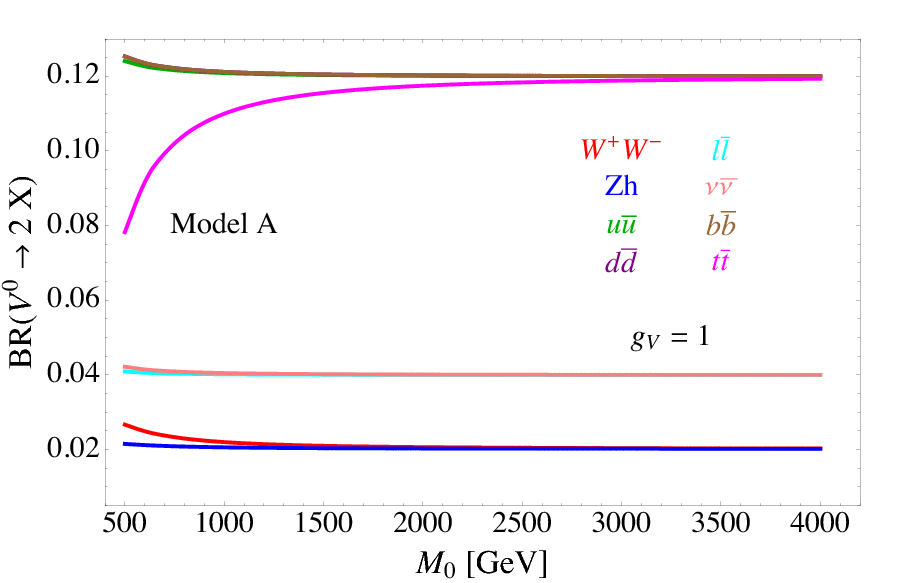
\includegraphics[width=.495\textwidth]{figures/Figures_BRWC.png}%
    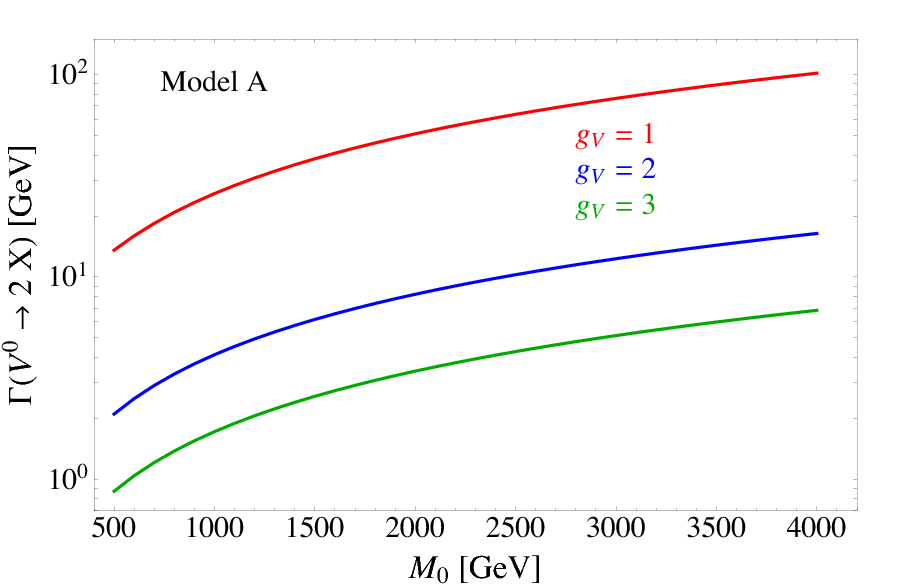
\includegraphics[width=.495\textwidth]{figures/Figures_WidthWC.png}
  \caption{HVT model A scenario: branching fractions for fermionic and bosonic decays when $g_V~=~1$ (left) as a function of the mass of the resonance $M_0$; total width of the resonance, as a function of its mass, considering different values of the parameter $g_V$ (right).~\cite{Pappadopulo2014}}
  \label{fig:HVT_modelA_BR_width}
\end{figure}

\subsection{Benchmark model B: strong coupling scenario}
\label{sec:theory_HVT_B}
In composite Higgs models~\cite{Contino2011}, the Higgs boson is the result of the spontaneous symmetry breaking of an $SO(5)$ symmetry to a $SO(4)$ group. New vector bosons are expected to appear, and the lightest ones can be represented by HVT model B when $c_H \sim c_F \sim 1$.\\ 
In this case:

\begin{equation}
\begin{split}
 & g_V c_H \approx -g_V,\\
 & g^2 c_F/g_V \approx g^2/g_V,\\
\end{split}
\label{eq:theory_HVT_modelB}
\end{equation}

\noindent hence the decay into bosons is not suppressed by $g_V$ parameter. In the benchmark scenario $g_V=3$, decays into dibosons are largely dominant, as it can be seen in fig.~\ref{fig:HVT_modelB_BR_width} (left); the total decay width increases for larger $g_V$ (fig.~\ref{fig:HVT_modelB_BR_width}, right). When the resonances start to be broad, \textit{i.e.} $\Gamma/M_V~\gg~10\%$, the assumptions leading to the simplified model are no longer valid, hence higher order, non-resonant effects must be taken into account.

\begin{figure}[!htb]
  \centering
    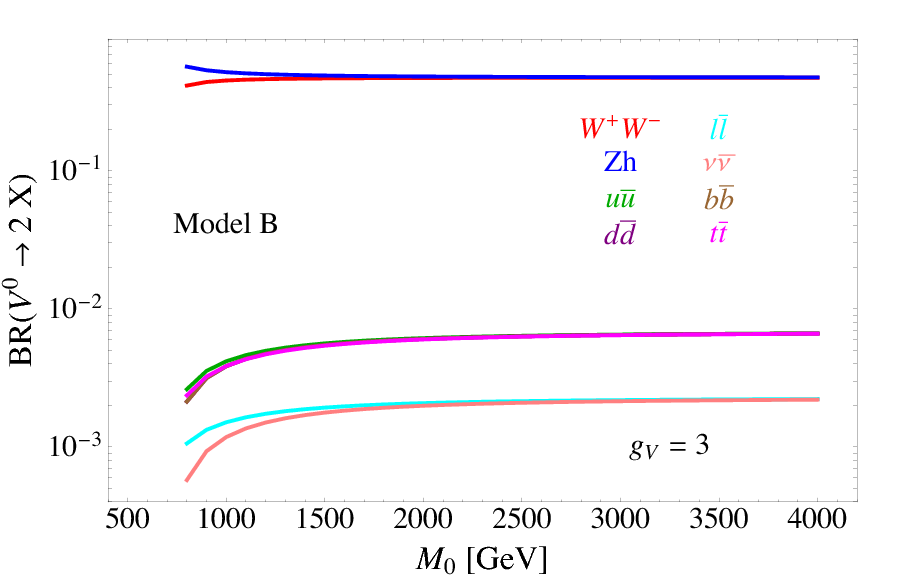
\includegraphics[width=.495\textwidth]{figures/Figures_BRSC.png}%
    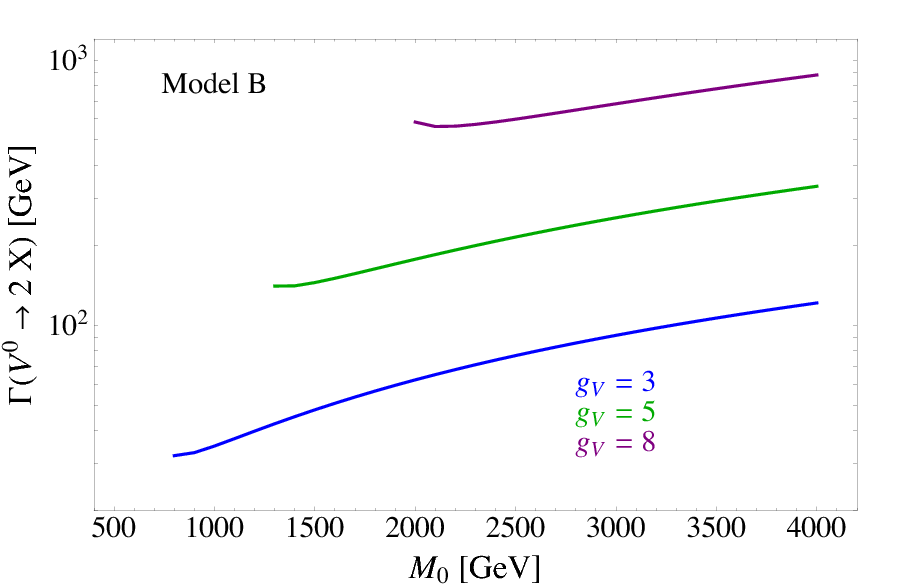
\includegraphics[width=.495\textwidth]{figures/Figures_WidthSC.png}
  \caption{HVT model B scenario: branching fractions for fermionic and bosonic decays when $g_V~=~3$ (left) as a function of the mass of the resonance $M_0$; total width of the resonance, as a function of its mass, considering different values of the parameter $g_V$ (right).~\cite{Pappadopulo2014}}
  \label{fig:HVT_modelB_BR_width}
\end{figure}

\subsection{HVT production}
\label{sec:theory_widths}
For resonance masses in the range of interest ($\sim$1 \TeV), the production mechanisms expected to be relevant are Drell-Yan (fig.~\ref{fig:theory_HVT_DY_prod}) and Vector Boson Fusion (VBF) (fig.~\ref{fig:theory_HVT_VBF_prod}).

\begin{figure}[!htb]
  \centering
\feynmandiagram [horizontal=a to b] {
  i1 [particle=\(q\)] -- [fermion] a -- [fermion] i2 [particle=\(\overline{q} \)],
  a -- [red!80!black, boson, edge label=\(V^{0}\), very thick] b,
  f1 [particle=\(\overline{\ell}\)] -- [fermion] b -- [fermion] f2 [particle=\(\ell\)],
};
%
\feynmandiagram [horizontal=a to b] {
  i1 [particle=\(q\)] -- [fermion] a -- [fermion] i2 [particle=\(\overline{q}'\)],
  a -- [red!80!black, boson, edge label=\(V^{-}\), very thick] b,
  f1 [particle=\(Z\)] -- [boson] b -- [boson] f2 [particle=\(W^{-}\)],
};
\caption{Examples of Drell-Yan production mechanism of a heavy $V$ HVT boson: $q$~--~$\bar{q}$ quark scattering producing a neutral $V^{0}$ that decays leptonically (left); $q$~--~$\bar{q}'$ scattering producing a charged $V^{-}$ that decays into a $W$ and $Z$ bosons (right).}
\label{fig:theory_HVT_DY_prod}
\end{figure}

% A bit uglier:
%
%\feynmandiagram [vertical'=a to c, horizontal=b to d] {
%a -- [boson, edge label=\(W^+\)] b,
%b -- [boson, edge label=\(W^-\)] c,
%b -- [red!80!black, boson, edge label=\(V^0\), very thick] d,
%f3 [particle=\(\overline f\)] -- [boson] d -- [boson] f4 [particle=\(f\)],
%
%i1 [particle=\(e^{-}\)]
%-- [fermion] a
%-- [fermion] f1 [particle=\(e^{-}\)],
%
%i2 [particle=\(e^{+}\)]
%-- [fermion] c
%-- [fermion] f2 [particle=\(e^{+}\)],
%};

%\feynmandiagram [vertical'=a to c, horizontal=b to d] {
%i1 [particle=\(e^{-}\)]
%-- [fermion] a
%-- [fermion] f1 [particle=\(e^{-}\)],
%
%i2 [particle=\(e^{+}\)]
%-- [fermion] c
%-- [fermion] f2 [particle=\(e^{+}\)],
%
%a -- [boson, edge label=\(W^+\)] b,
%b -- [boson, edge label=\(W^-\)] c,
%b -- [red!80!black, boson, edge label=\(V^0\), very thick] d,
%
%};
\begin{figure}[!htb]
  \centering
\begin{tikzpicture}
\begin{feynman}
\vertex (e);
\vertex [right=of e] (v); % vertice del bosone V0
\vertex [above right=of v] (m) {\( Z \)};
%\vertex [below right=of v] (n) {\( h \)};%in h
\vertex [below right=of v] (n) {\( W^{+} \)};%in W
\vertex [above left=of e] (c) {\( W^{+} \)};
\vertex [above left=of c] (a);
\vertex [right=of c] (f);

%\vertex [below left=of e] (d) {\( W^{-} \)};%W
\vertex [below left=of e] (d) {\( Z \)};%Z
\vertex [below left=of d] (b);
\vertex [right=of d] (g);

\diagram* {
(c) -- [boson, edge label'=\(\)] (e), %il bosone collega il vertice (c) col vertice (e) 
(d) -- [boson, edge label=\(\)] (e), %il bosone collega il vertice (d) col vertice (e) W^{-}
%(e) -- [red!80!black!, boson, edge label=\(V^0\), very thick] (v), %il bosone collega il vertice (e) col vertice (v)%V0
(e) -- [red!80!black!, boson, edge label=\(V^+\), very thick] (v), %il bosone collega il vertice (e) col vertice (v)%V+
(v) -- [boson, edge label'=\(\)] (m),
%(v) -- [scalar, edge label=\(\)] (n),%h
(v) -- [boson, edge label=\(\)] (n),%W
(a) -- [fermion, edge label=\(u\)] (c),
(b) -- [fermion, edge label=\(d\)] (d),
(c) -- [fermion, edge label=\(d\)] (f),
%(d) -- [fermion, edge label=\(u\)] (g),%u
(d) -- [fermion, edge label=\(d\)] (g),%d

};
\end{feynman}
\end{tikzpicture}
\caption{Example of VBF production mechanism of a heavy $V$ HVT boson: a charged $V^+$ boson is produced by a couple of $W$ and \Z bosons, as a result of electroweak interactions of initial state $u$ and $d$ quarks. $V^+$ decays into a $Z$ boson and a $W^{+}$ boson. The final state signature includes the presence of a pair of quarks, due to the primary interactions.}
\label{fig:theory_HVT_VBF_prod}
\end{figure}

\noindent The cross-section of the production mechanisms is given by:

\begin{equation}
\sigma (pp \rightarrow V + X) = \left. \sum_{i, j \in p} \frac{\Gamma_{V \rightarrow ij}}{M_V} f(J, S_i, S_j) g(C_i, C_j) \frac{dL_{ij}}{d\hat{s}} \right|_{\hat{s} = M_V^2},
\label{eq:prod_xsec}
\end{equation}

\noindent where $i$, $j$ are the partons (or the vector bosons) involved in the hard interaction, $\Gamma_{V \rightarrow ij}$ is the partial width of the process $V \rightarrow ij$, $f(J, S_i, S_j)$ is a function of the spin of the resonance and of the partons (or vector bosons), $g(C_i, C_j)$ is a function of the colour factors of each parton, $\hat{s}$ is the center-of-mass energy at parton level and $\frac{dL_{ij}}{d \hat{s}}$ are the parton luminosities, that are independent from HVT model (that enters only in $\Gamma_{V \rightarrow ij}$). The vector bosons can be treated as partons inside the proton, under the Effective $W$ Approximation~\cite{Dawson:1984gx}.
\\
Parton luminosities, calculated for a center-of-mass energy of 14 TeV starting from quark and antiquark parton distribution functions (PDF), are displayed in fig.~\ref{fig:HVT_DY_partolumi} (Drell-Yan mechanism) and~\ref{fig:HVT_VBF_partolumi} (VBF mechanism). VBF luminosities are suppressed by the $\alpha_{\text{weak}}$ factor, therefore the process is relevant only when the bosonic decays of the triplet are dominant (strongly coupled scenario). 
\begin{figure}[!htb]
  \centering
    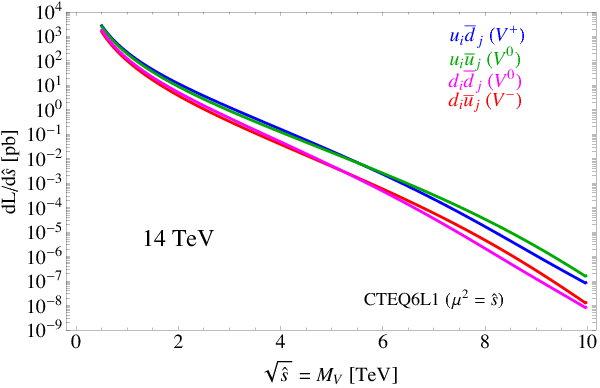
\includegraphics[width=.495\textwidth]{figures/Figures_LumiDY14.png}
  \caption{Parton luminosities for Drell-Yan production process of a heavy $V$ HVT boson, as a result of the scattering between $i$ and $j$ partons, as a function of the parton center-of-mass energy, for the LHC proton-proton collisions performed at 14 TeV.~\cite{Pappadopulo2014}}
  \label{fig:HVT_DY_partolumi}
\end{figure}

\begin{figure}[!htb]
  \centering
    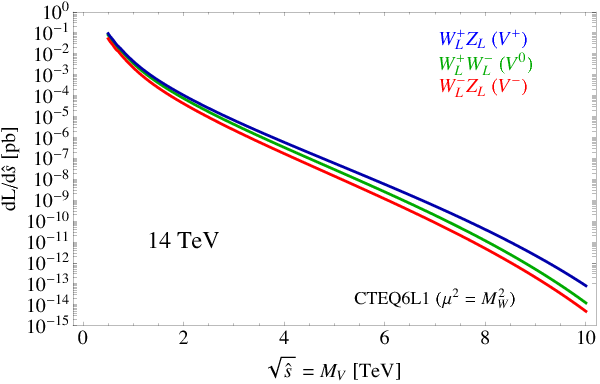
\includegraphics[width=.495\textwidth]{figures/Figures_LumiVBF14.png}
  \caption{Parton luminosities for VBF production process of a heavy $V$ HVT boson, as a result of the scattering between longitudinally polarized vector bosons, as a function of the parton center-of-mass energy, for the LHC proton-proton collisions performed at 14 TeV.~\cite{Pappadopulo2014}}
  \label{fig:HVT_VBF_partolumi}
\end{figure}

\clearpage

\subsection{Search for HVT resonances at LHC}
\label{sec:theory_HVT_limits_LHC}
No evidence of HVT resonances has been observed so far at the LHC experiments. Data collected by the ATLAS and CMS detectors are used to set limits on the HVT resonance masses and coupling parameters. Experimental results from proton-proton collisions performed at a center-of-mass energy of 8 TeV (Run 1 era) at the LHC brought to the following conclusions. A weakly coupled resonance, in the context of benchmark model A ($g_V = 1$) was excluded up to 3 TeV by Run 1 data. By looking at parton luminosities in fig.\ref{fig:HVT_DY_partolumi}, under the hypothesis of LHC proton-proton collisions at a center-of-mass energy of 14 \TeV, the sensitivity is expected to increase up to $m_V \approx 6$ TeV, once data are collected for an integrated luminosity of 300 $\mbox{fb}^{-1}$. A strongly coupled resonance, in the context of benchmark model B ($g_V = 3$) is excluded up to 2 TeV by Run 1 data. Data produced by LHC at 14 TeV should increase the sensitivity up to $m_V \approx 3-4$ TeV.\\
The most stringent limits are provided by the latest data produced by LHC at a center-of-mass energy of 13 TeV (Run 2 era).

\vspace*{1\baselineskip}

\noindent Numerous searches for HVT triplet have been performed at the CMS experiment in different final states: the most sensitive ones were those in all-hadronic topology. The analysis searching for $WW$, $WZ$, $ZZ$ resonances in the $q\bar{q}q\bar{q}$ final state~\cite{Sirunyan:2017acf,bib:CMS-PAS-B2G-17-001} excludes a $W'$ with mass below 3.6~\TeV and a $Z'$ with mass below 2.7~\TeV in the model B scenario (fig.~\ref{fig:theory_B2G-17-001}). The analysis searching for $WH$, $ZH$ resonances in the $q\bar{q} b \bar{b}$ final state~\cite{CMS:2017eme,bib:CMS-PAS-B2G-17-002} excludes a $W'$ lighter than 2.97 (3.15) TeV in the HVT model A (model B), and a $Z'$ up to 1.67 (2.26) TeV in HVT model A (model B) (fig.~\ref{fig:theory_B2G-17-002}). In fig.~\ref{fig:theory_exclusion_parameter_plane}, results of \cite{Sirunyan:2017acf,bib:CMS-PAS-B2G-17-001} (left) and \cite{CMS:2017eme,bib:CMS-PAS-B2G-17-002} (right) searches are interpreted as exclusion contours in the coupling parameters plane of the HVT model ($g_Vc_H$ and $g^2 c_F/g_V$). In the gray shaded area, the narrow width approximation fails. The coloured curves display the parameter exclusion for different mass hypotheses of the triplet. Coloured markers show the model A and B benchmark scenarios.

\begin{figure}[!htb]
  \centering
    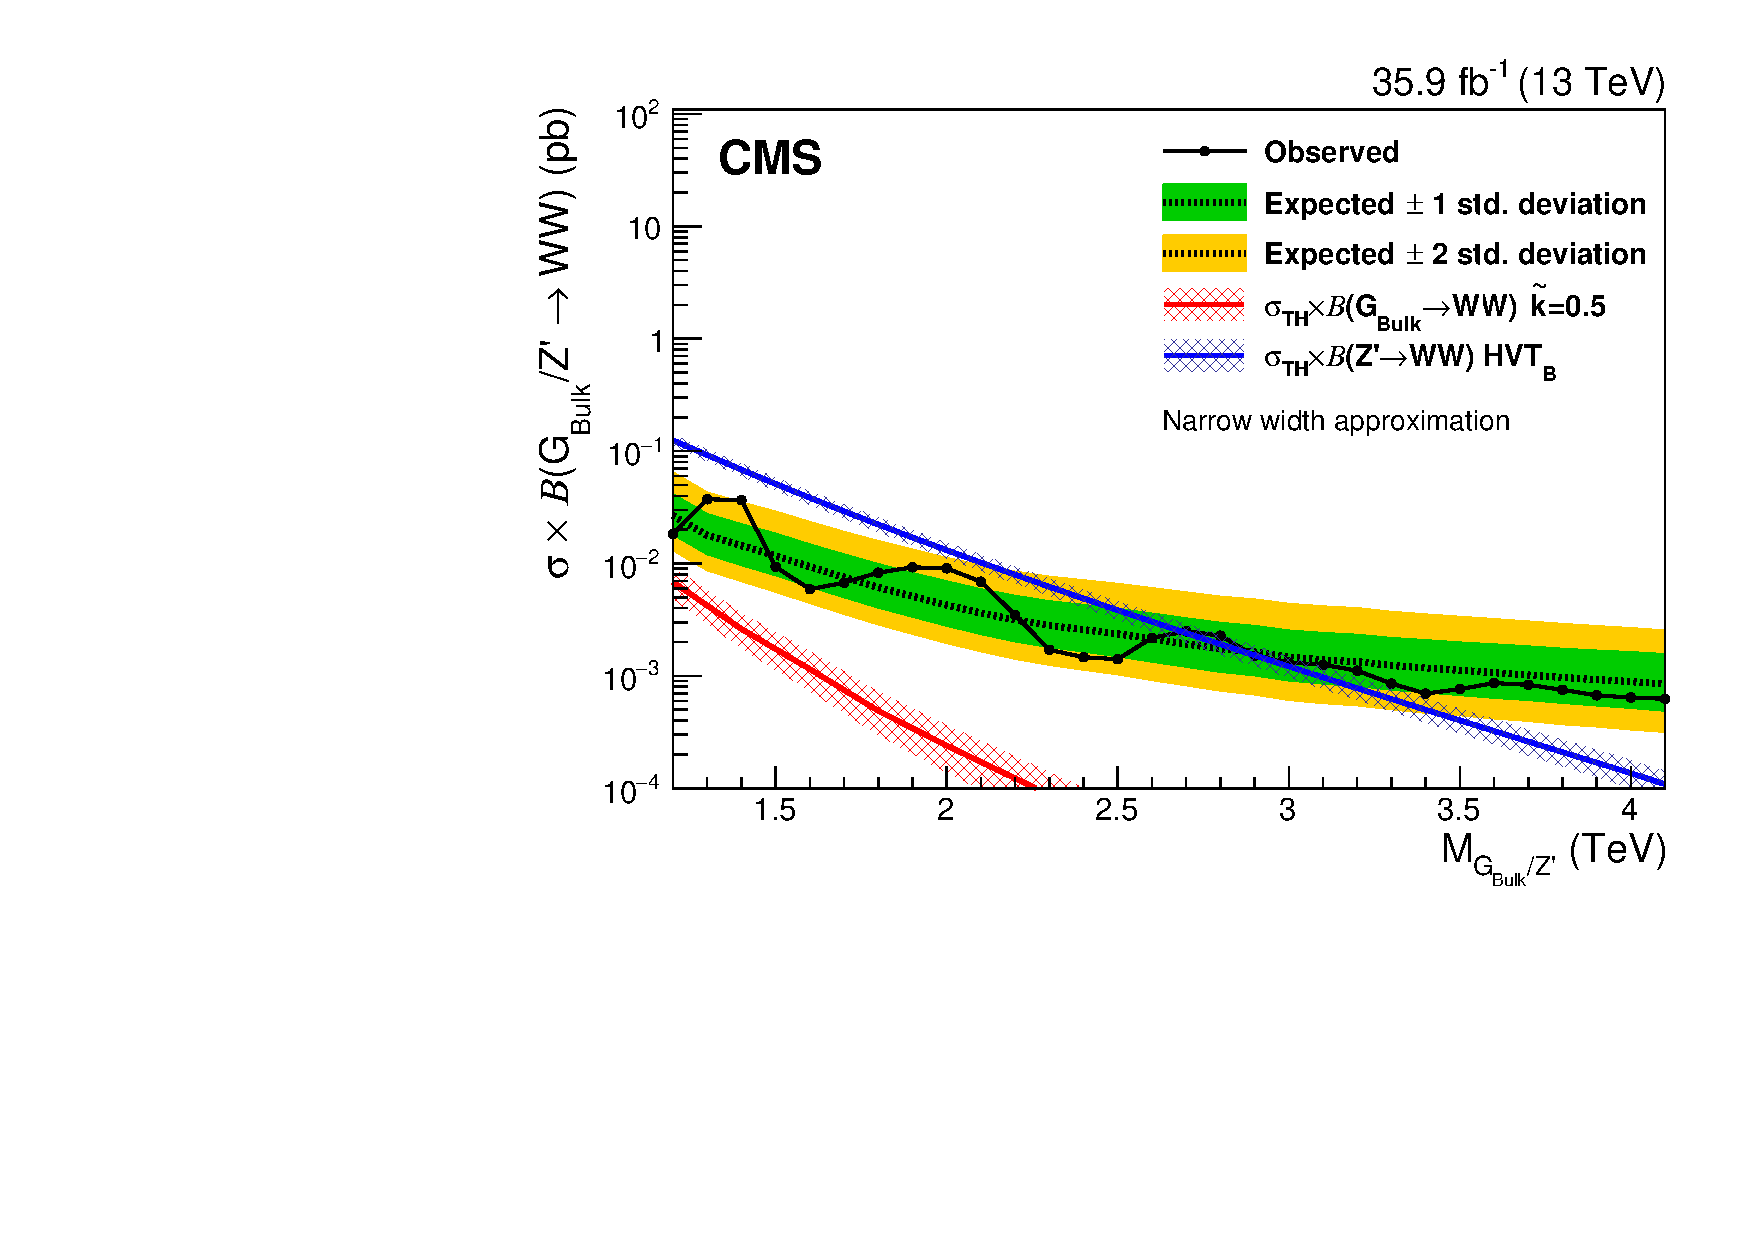
\includegraphics[width=.495\textwidth]{figures/B2G-17-001/CMS-B2G-17-001_Figure_006-a.pdf}%
    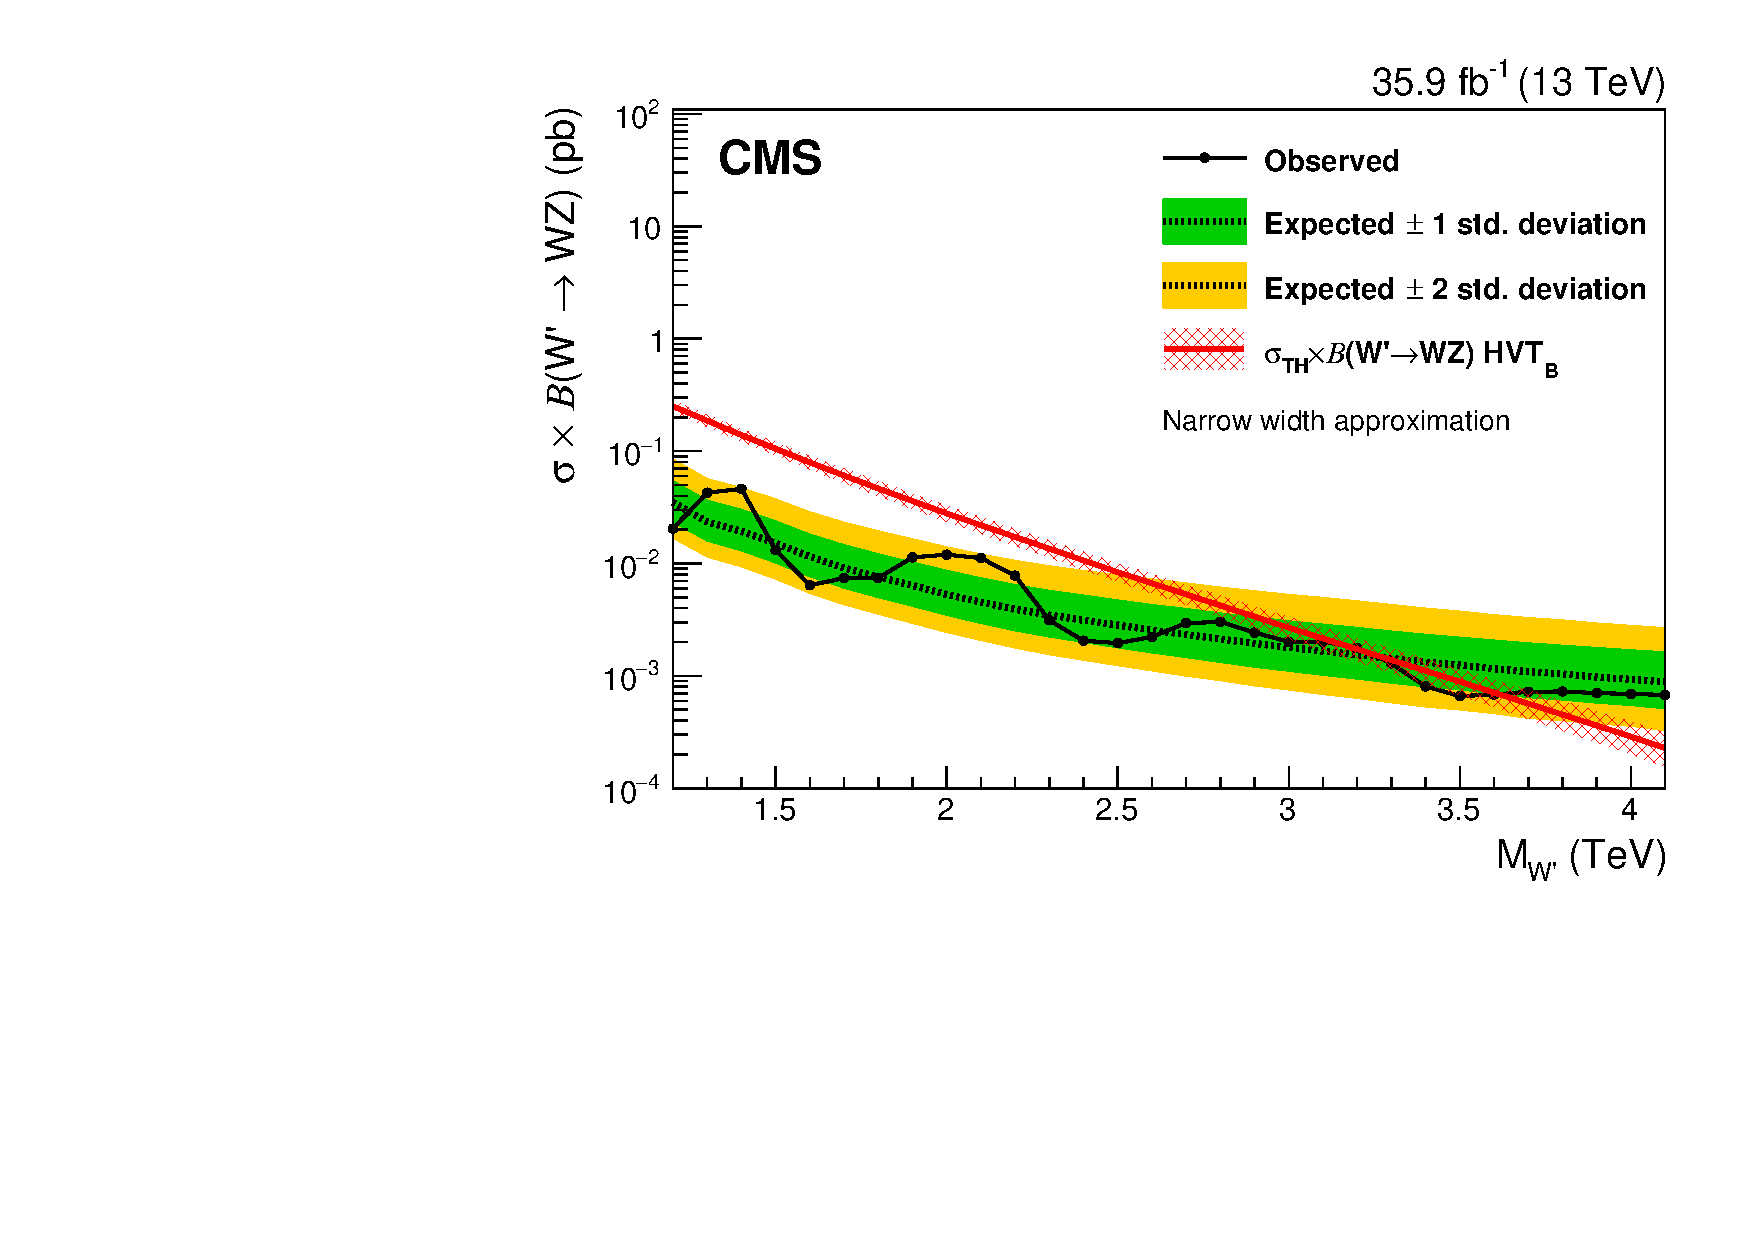
\includegraphics[width=.495\textwidth]{figures/B2G-17-001/CMS-B2G-17-001_Figure_006-b.pdf}
  \caption{The observed and expected limits, with 68\% and 95\% uncertainty bands, on the product of the cross-section and branching fraction $\sigma \mathcal{B} (Z' \rightarrow WW)$ for a spin-1 $Z'$ (left) and $\sigma \mathcal{B} (W' \rightarrow WZ)$ for a spin-1 $W'$ (right), as a function of the reconstructed mass of the diboson resonance. The coloured lines show the theoretical predictions for the HVT model B.~\cite{Sirunyan:2017acf,bib:CMS-PAS-B2G-17-001}}
  \label{fig:theory_B2G-17-001}
\end{figure}

\begin{figure}[!htb]
  \centering
    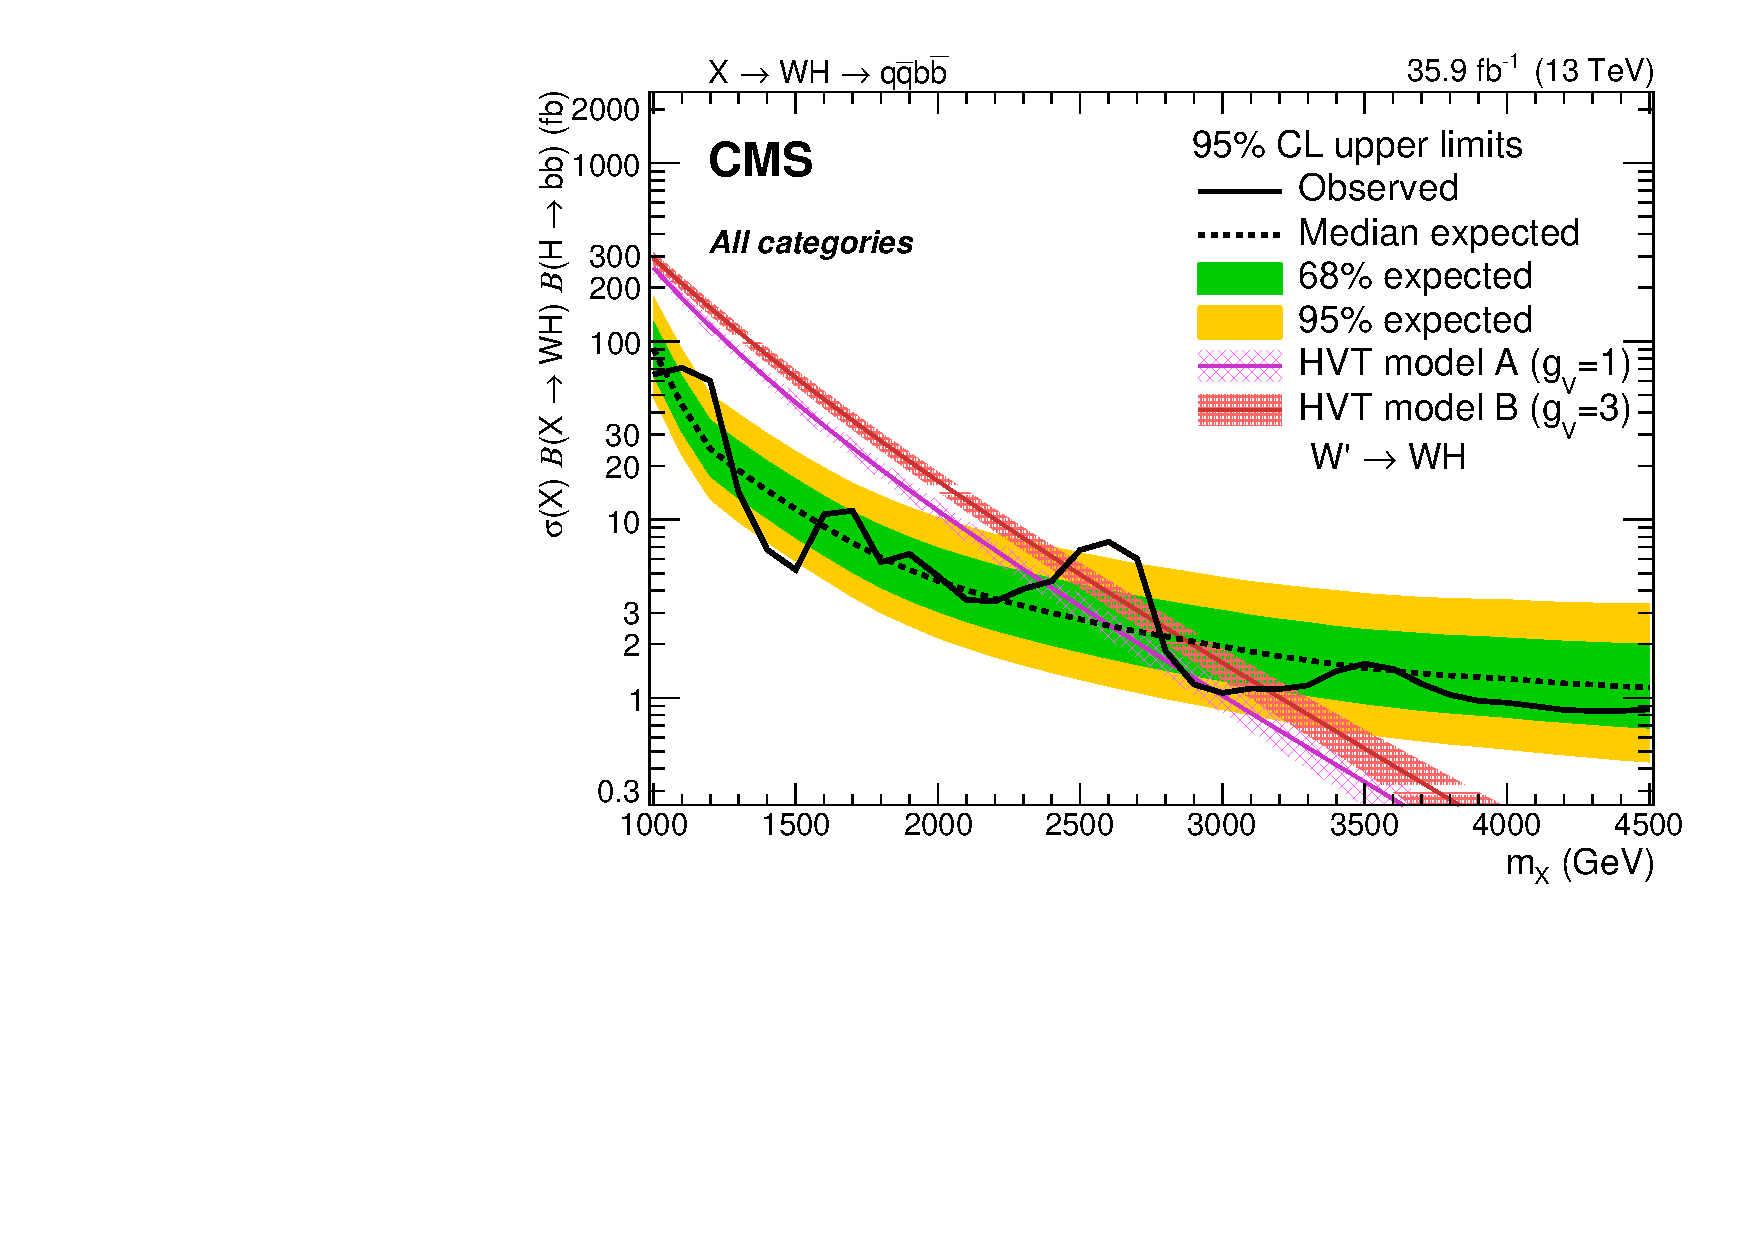
\includegraphics[width=.495\textwidth]{figures/B2G-17-002/CMS-B2G-17-002_Figure_005-a.pdf}%
    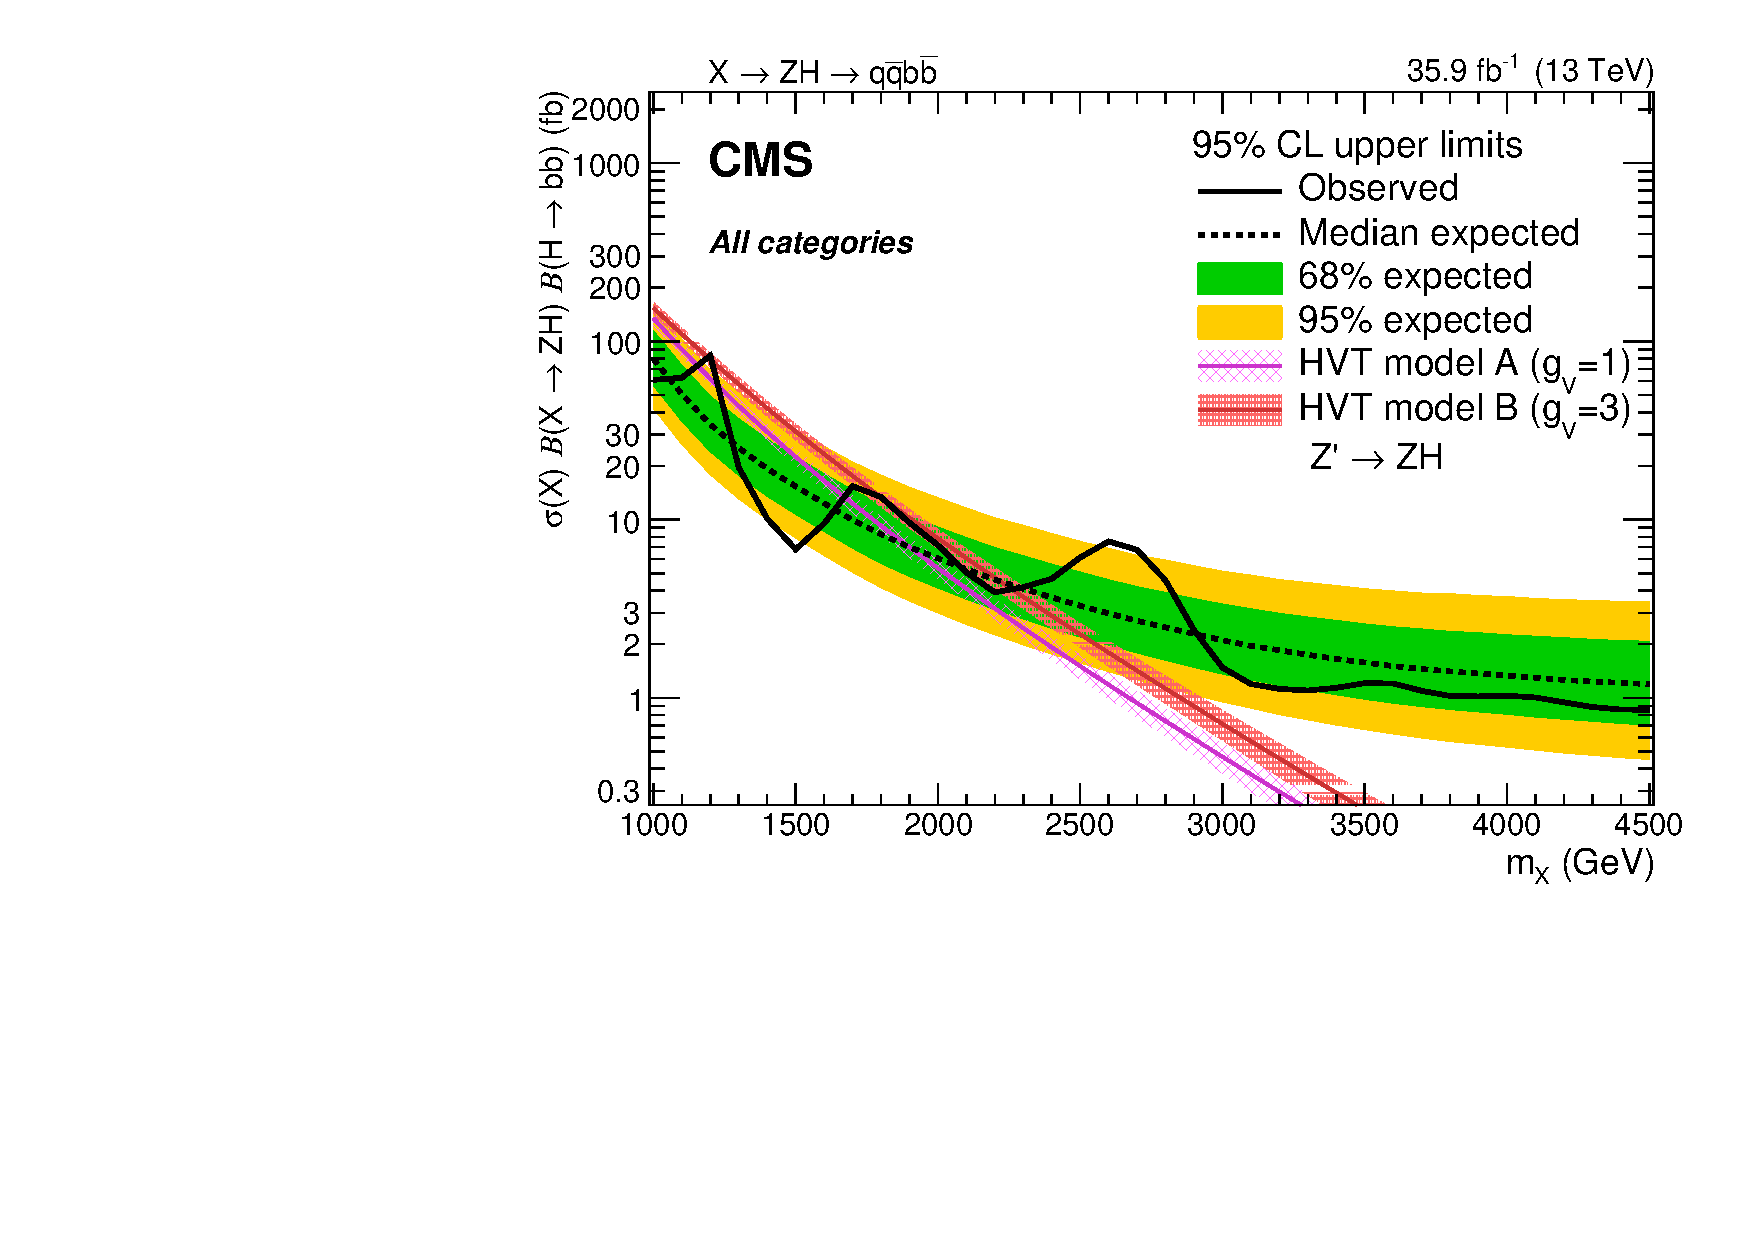
\includegraphics[width=.495\textwidth]{figures/B2G-17-002/CMS-B2G-17-002_Figure_005-b.pdf}
  \caption{The observed and expected limits, with 68\% and 95\% uncertainty bands, on the product of the cross-section and branching fraction $\sigma \mathcal{B} (W' \rightarrow WH)$ for a spin-1 $W'$ (left) and $\sigma \mathcal{B} (Z' \rightarrow ZH)$ for a spin-1 $Z'$ (right), as a function of the reconstructed mass of the diboson resonance. The coloured lines show the theoretical predictions for the HVT model A and B.~\cite{CMS:2017eme,bib:CMS-PAS-B2G-17-002}}
  \label{fig:theory_B2G-17-002}
\end{figure}

\begin{figure}[!htb]
  \centering
    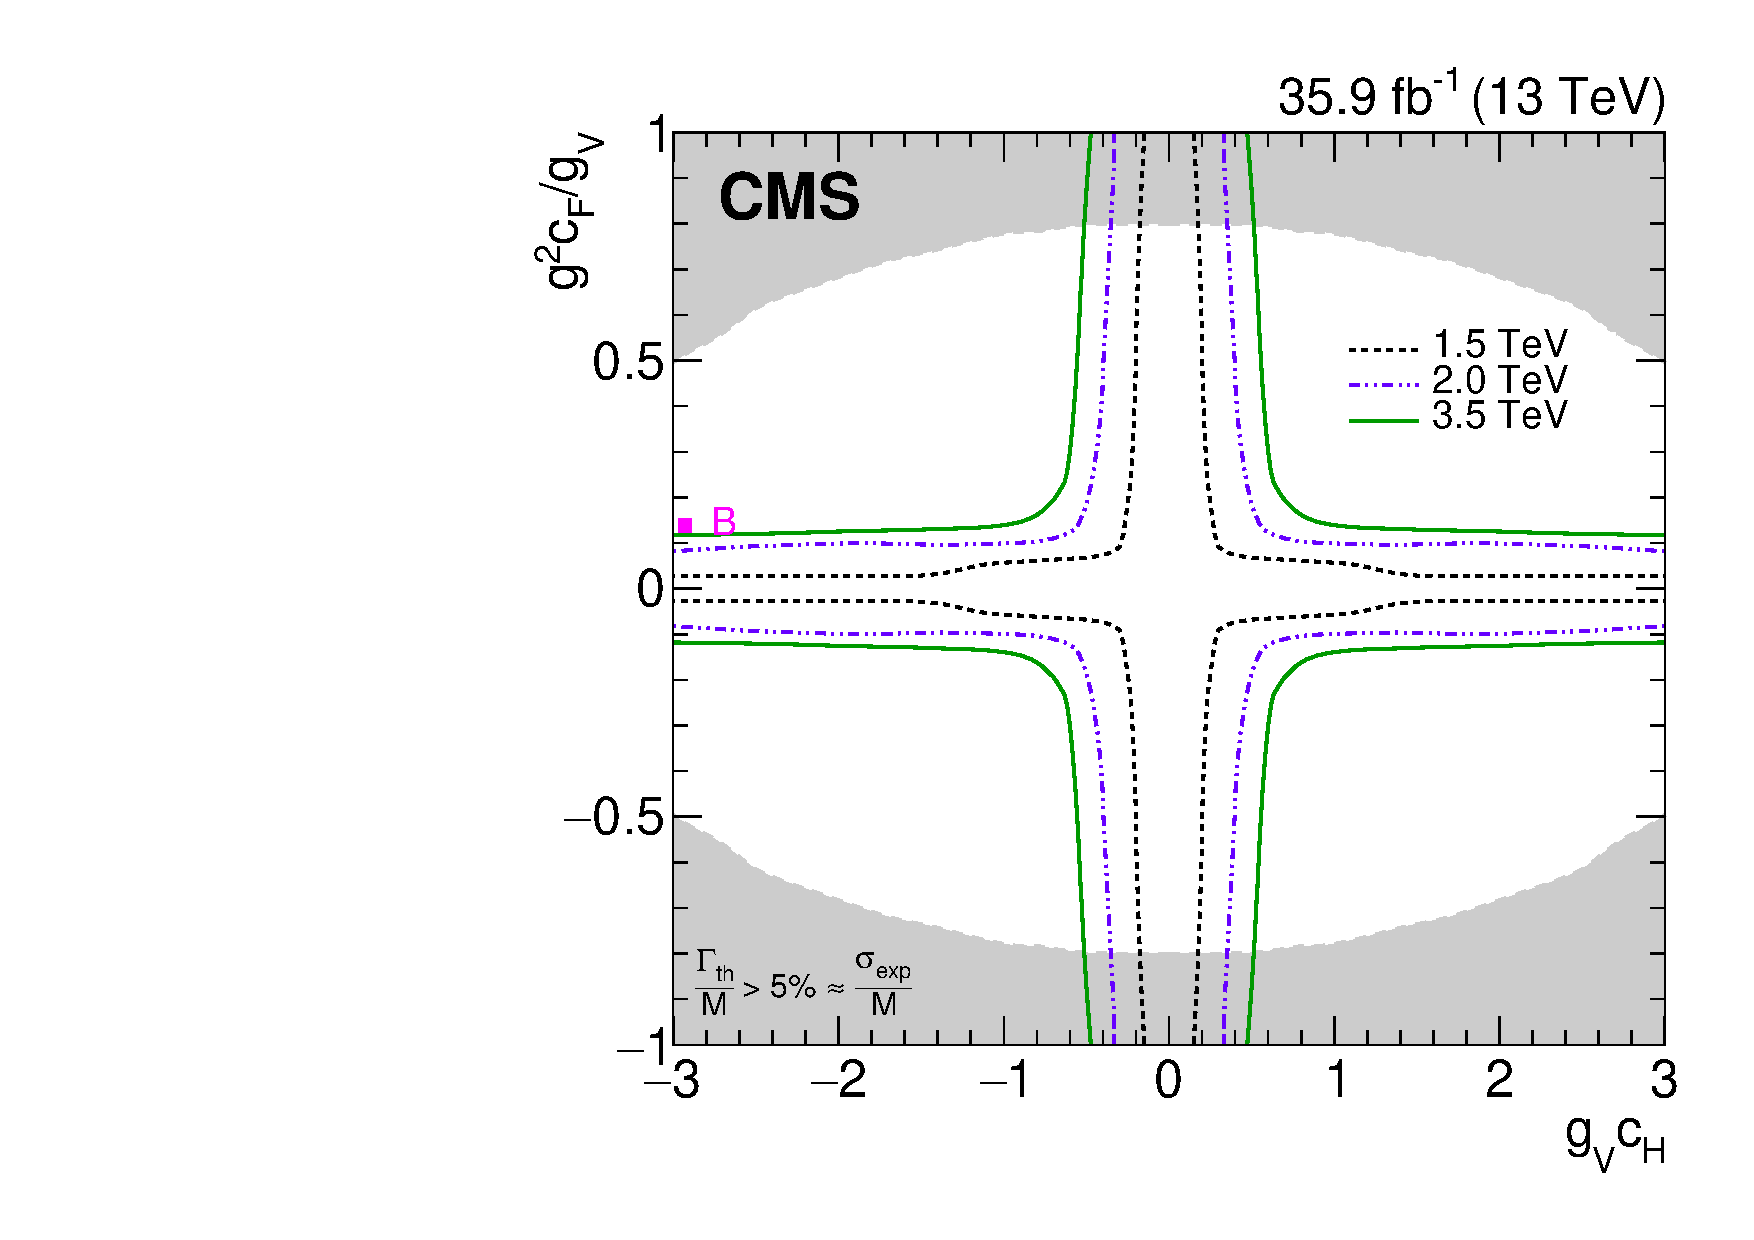
\includegraphics[height=.4\textwidth]{figures/B2G-17-001/CMS-B2G-17-001_Figure_007.pdf}%
    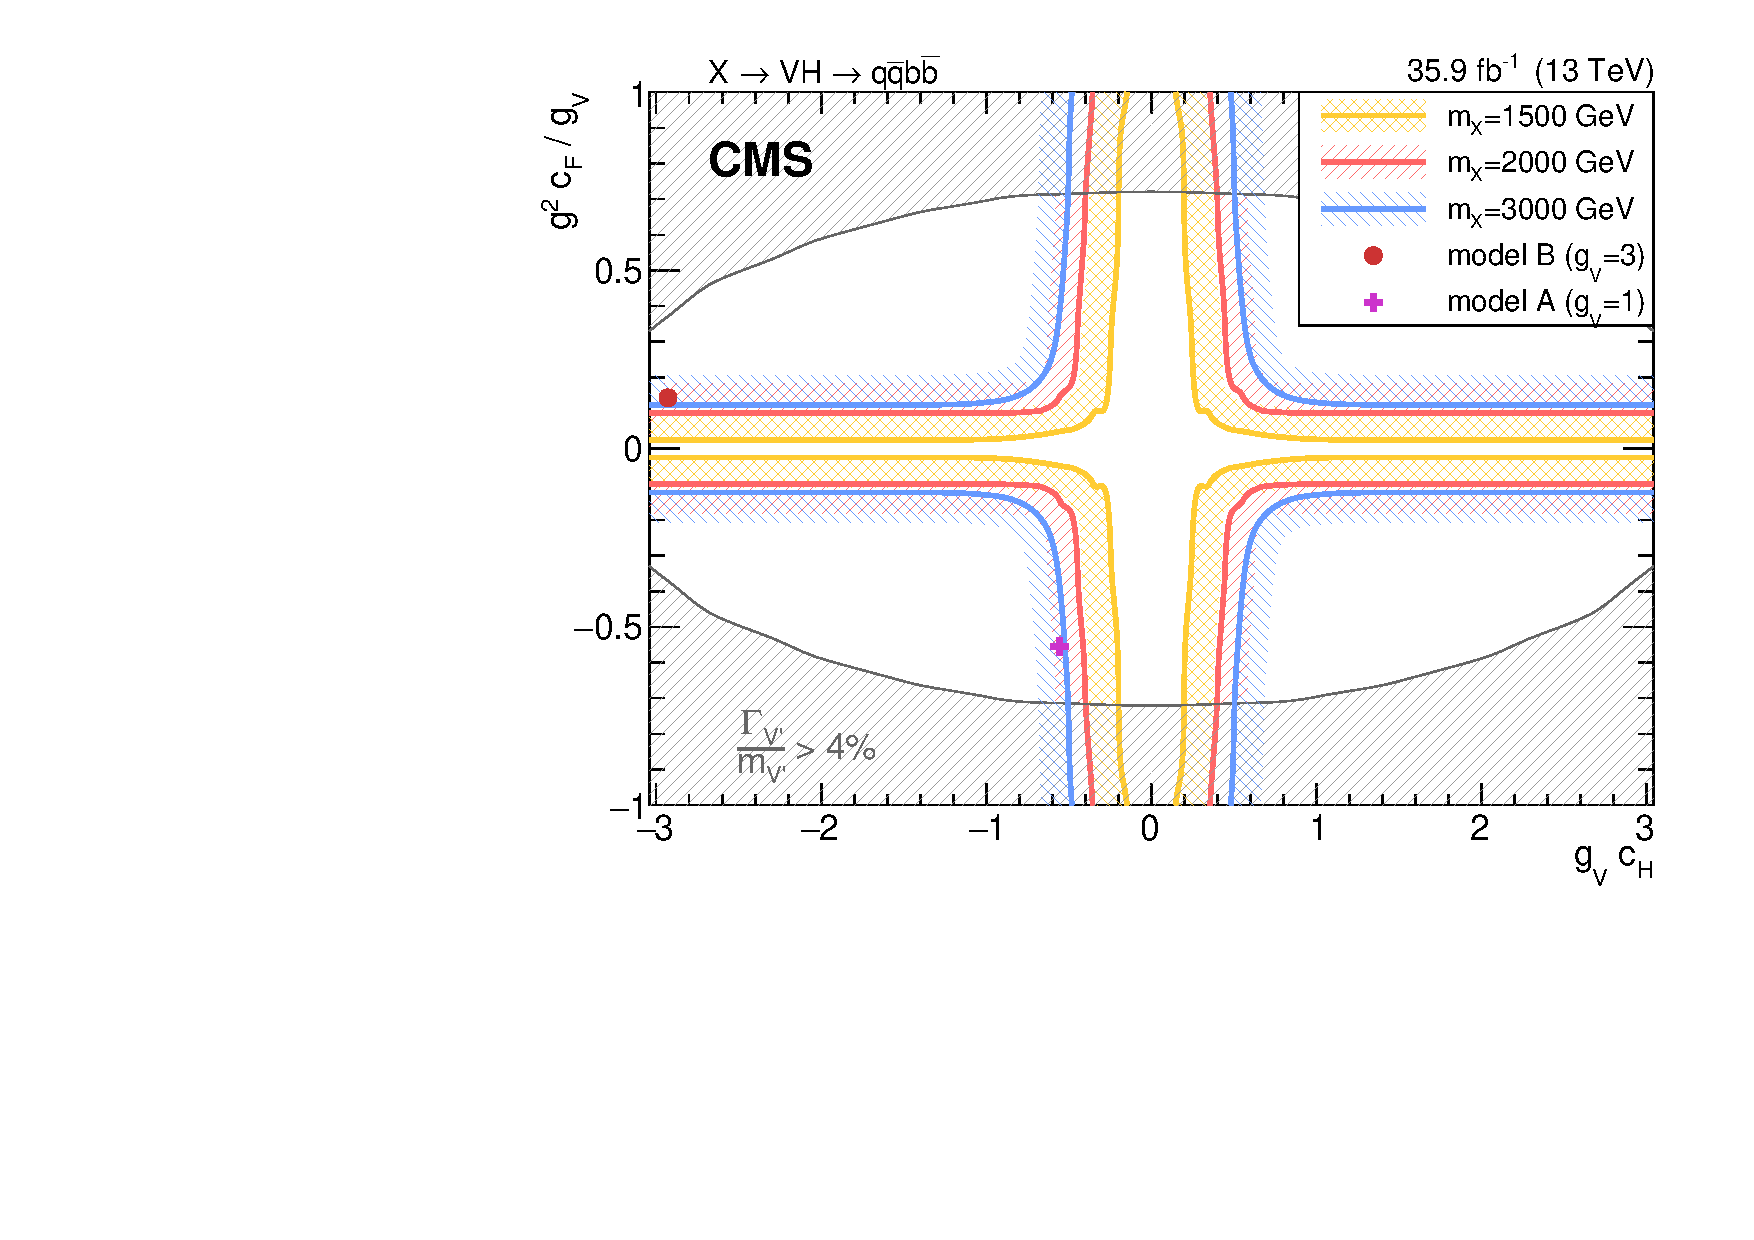
\includegraphics[height=.4\textwidth]{figures/B2G-17-002/CMS-B2G-17-002_Figure_007.pdf}
  \caption{Exclusion contours in the coupling parameters plane of the HVT model ($g_Vc_H$ and $g^2 c_F/g_V$), for~\cite{Sirunyan:2017acf,bib:CMS-PAS-B2G-17-001} analysis (left), and~\cite{CMS:2017eme,bib:CMS-PAS-B2G-17-002} analysis (right).}
  \label{fig:theory_exclusion_parameter_plane}
\end{figure}

\clearpage

\noindent Many other final states have been exploited at CMS: $ZW, ZZ \rightarrow \ell \bar{\ell} q\bar{q}$~\cite{CMS-PAS-B2G-17-013}; $WH, ZH \rightarrow (\ell \bar{\ell}, \ell \nu, \nu \bar{\nu}) b \bar{b}$~\cite{Khachatryan:2016cfx}; $WZ, WW \rightarrow \ell \nu q \bar{q}$~\cite{CMS-PAS-B2G-16-029}; $HH \rightarrow b \bar{b} \tau^+ \tau^-, (WH, ZH) \rightarrow q \bar{q} \tau^+ \tau^-$~\cite{CMS-PAS-B2G-17-006}. Finally, $ZW, ZZ \rightarrow \nu \bar{\nu} q \bar{q}$~\cite{CMS-PAS-B2G-17-005} results will be extensively described in this thesis. 

\vspace*{1\baselineskip}

%Revision
%
\noindent The results (or preliminary results) on HVT searches in diboson final states, performed with 2016 data and published by the CMS Collaboration so far, are summarized in fig.~\ref{fig:theory_CMS_Diboson_Summary_HVT}. 
%The dark orange curve corresponds to the $(WZ, WW) \rightarrow q\bar{q}q\bar{q}$ analysis~\cite{Sirunyan:2017acf,bib:CMS-PAS-B2G-17-001}; the light blue curve corresponds to the $(WH, ZH) \rightarrow q\bar{q} b \bar{b}$ analysis~\cite{CMS:2017eme,bib:CMS-PAS-B2G-17-002}; the light orange curve corresponds to the analysis discussed in this thesis~\cite{CMS-PAS-B2G-17-005}.

\begin{figure}[!htb]
  \centering
    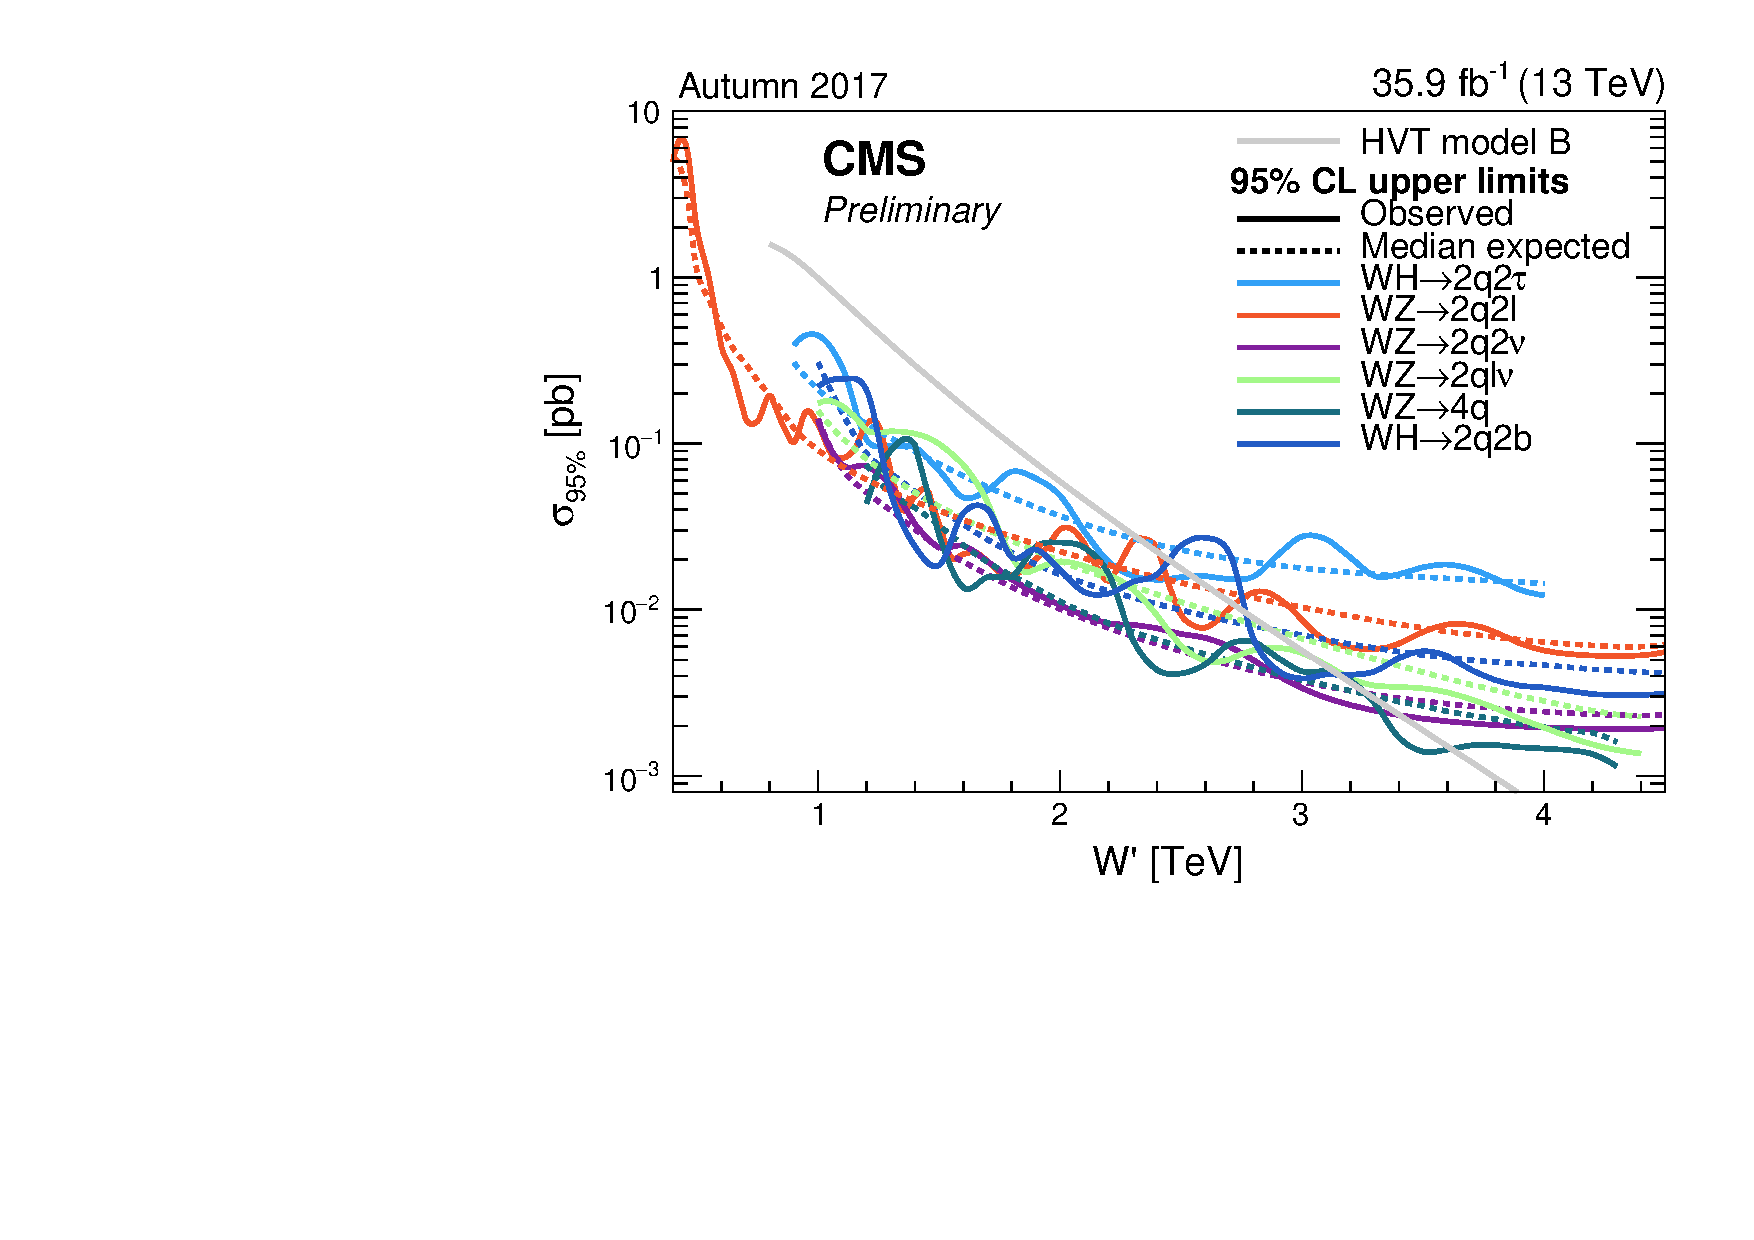
\includegraphics[width=.495\textwidth]{figures/Autumn2017/combiLimitsWprime_HVTB.pdf}%
    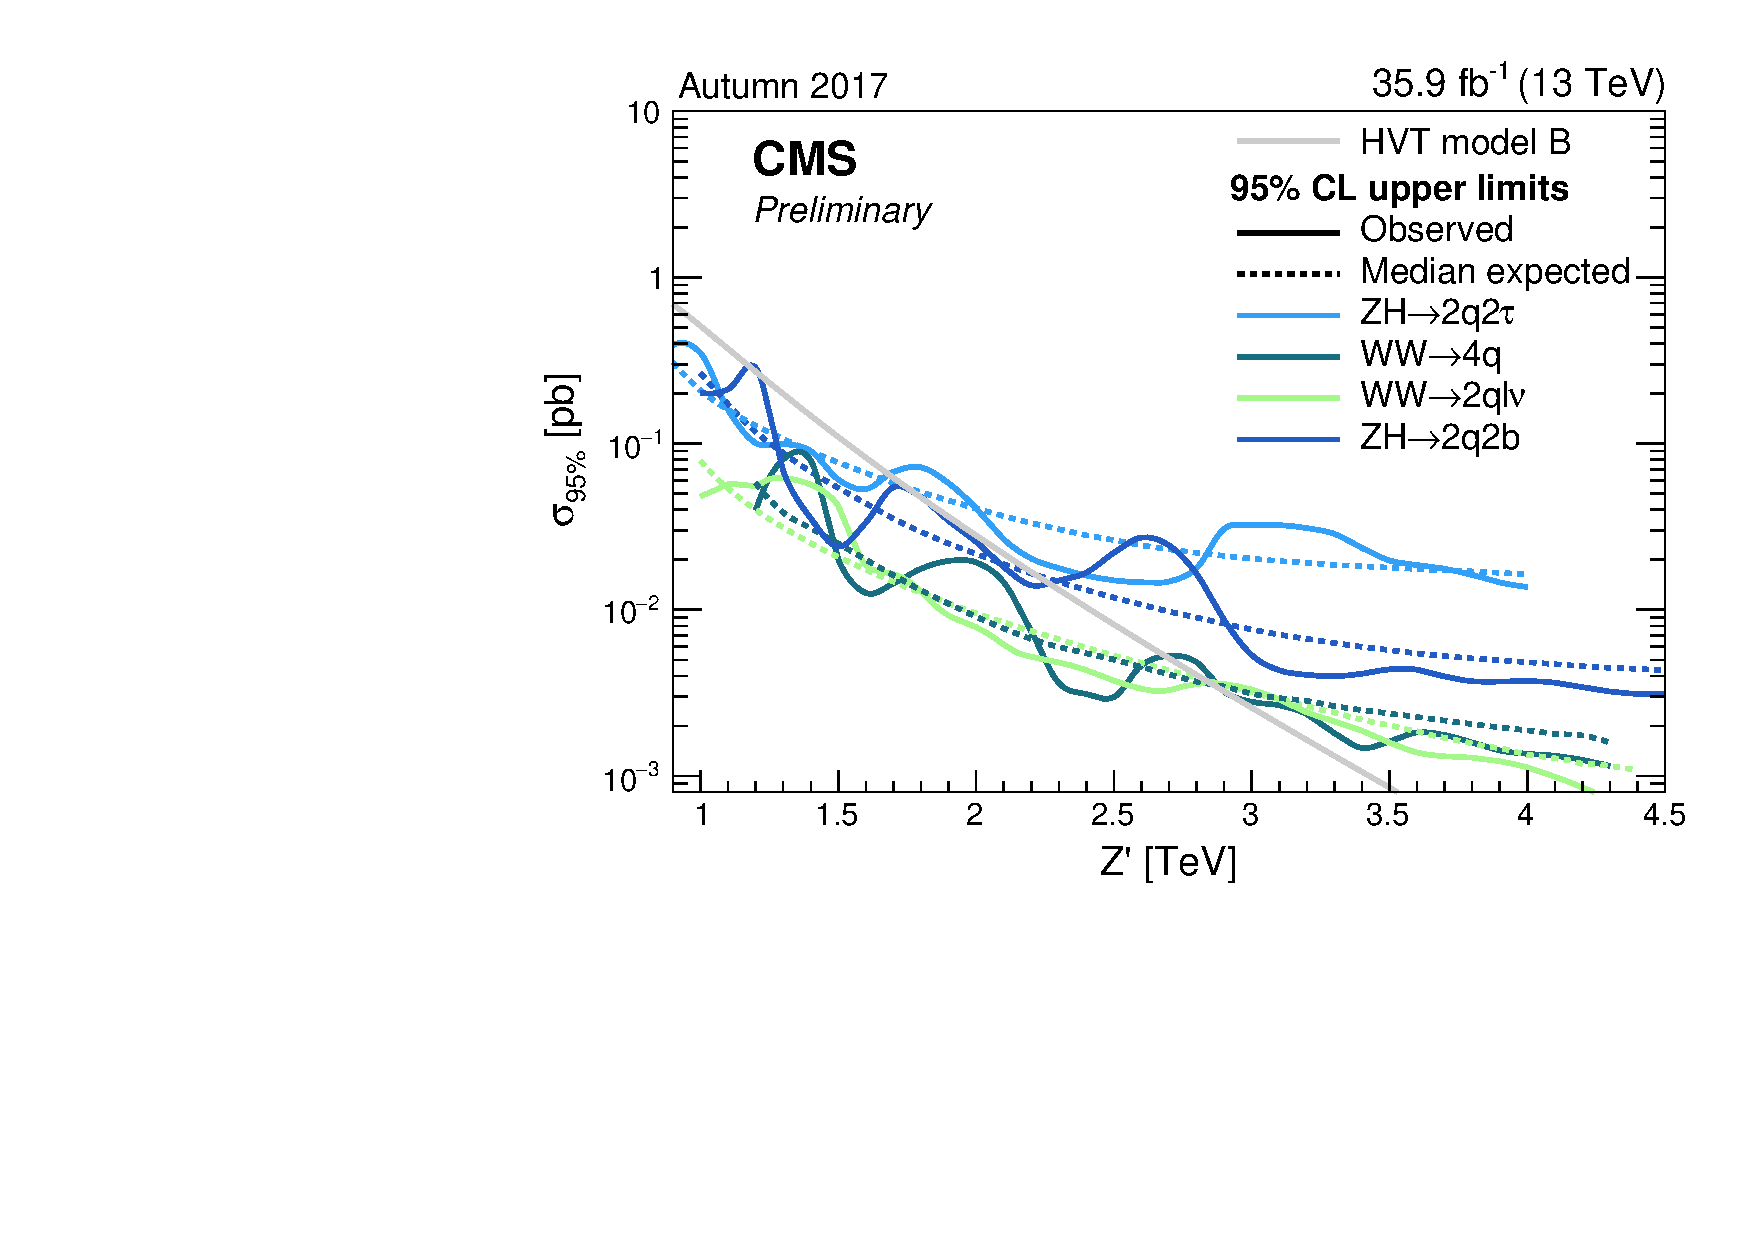
\includegraphics[width=.495\textwidth]{figures/Autumn2017/combiLimitsZprime_HVTB.pdf}
  \caption{The observed and expected limits on the product of the cross-section and branching fraction $\sigma \mathcal{B} (W' \rightarrow (WZ, WH))$ for a spin-1 $W'$ (left) and $\sigma \mathcal{B} (Z' \rightarrow (ZH, WW))$ for a spin-1 $Z'$ (right), as a function of the reconstructed mass of the diboson resonance.~\cite{CMSDibPublicResults} The gray line shows the theoretical prediction for the HVT model B. The light blue curve corresponds to the $HH \rightarrow b \bar{b} \tau^+ \tau^-, (WH, ZH) \rightarrow q \bar{q} \tau^+ \tau^-$ analysis~\cite{CMS-PAS-B2G-17-006}; the dark orange curve corresponds to the $ZW, ZZ \rightarrow \ell \bar{\ell} q\bar{q}$ analysis~\cite{CMS-PAS-B2G-17-013}; the light green curve corresponds to the $WZ, WW \rightarrow \ell \nu q \bar{q}$ analysis~\cite{CMS-PAS-B2G-16-029}; the dark green curve corresponds to the $(WZ, WW) \rightarrow q\bar{q}q\bar{q}$ analysis~\cite{Sirunyan:2017acf,bib:CMS-PAS-B2G-17-001}; the dark blue curve corresponds to the $(WH, ZH) \rightarrow q\bar{q} b \bar{b}$ analysis~\cite{CMS:2017eme,bib:CMS-PAS-B2G-17-002}; finally, the violet curve corresponds to the analysis discussed in this thesis~\cite{CMS-PAS-B2G-17-005}.}
  \label{fig:theory_CMS_Diboson_Summary_HVT}
\end{figure}


%\clearpage

\noindent Searches for HVT model B resonances have been performed at the ATLAS experiment as well. Results for a $W' \rightarrow WZ$ reported in fig.~\ref{fig:theory_ATLAS_Diboson_Summary} include the searches performed in $WW, WZ, ZZ \rightarrow q \bar{q} q \bar{q}$ final state~\cite{Aaboud:2017eta}; $WZ, WW \rightarrow \ell \nu q \bar{q}$ final state~\cite{ATLAS-CONF-2017-051}; $ZW, ZZ \rightarrow (\ell \bar{\ell}, \ell \nu, \nu \bar{\nu}) q \bar{q}$ final state~\cite{ATLAS-CONF-2016-082}. The all-hadronic final state has the best sensitivity and it excludes a $W'$ resonance up to 3.3 TeV (model B scenario). Results for a $W' \rightarrow WH$ and for a $Z' \rightarrow ZH$ are displayed in fig.~\ref{fig:theory_ATLAS_Diboson_Summary_VH} (left and right respectively), and they include searches performed in $WH, ZH \rightarrow q \bar{q} b \bar{b}$ final state~\cite{Aaboud:2017ahz}, and $WH, ZH \rightarrow \ell \bar{\ell}, \ell \nu, \nu \bar{\nu}) b \bar{b}$~\cite{ATLAS-CONF-2017-055}. A $W'$ is excluded up to 2.9 TeV and a $Z'$ is excluded up to 2.8 TeV (in the model B scenario).

\begin{figure}[!htb]
  \centering
    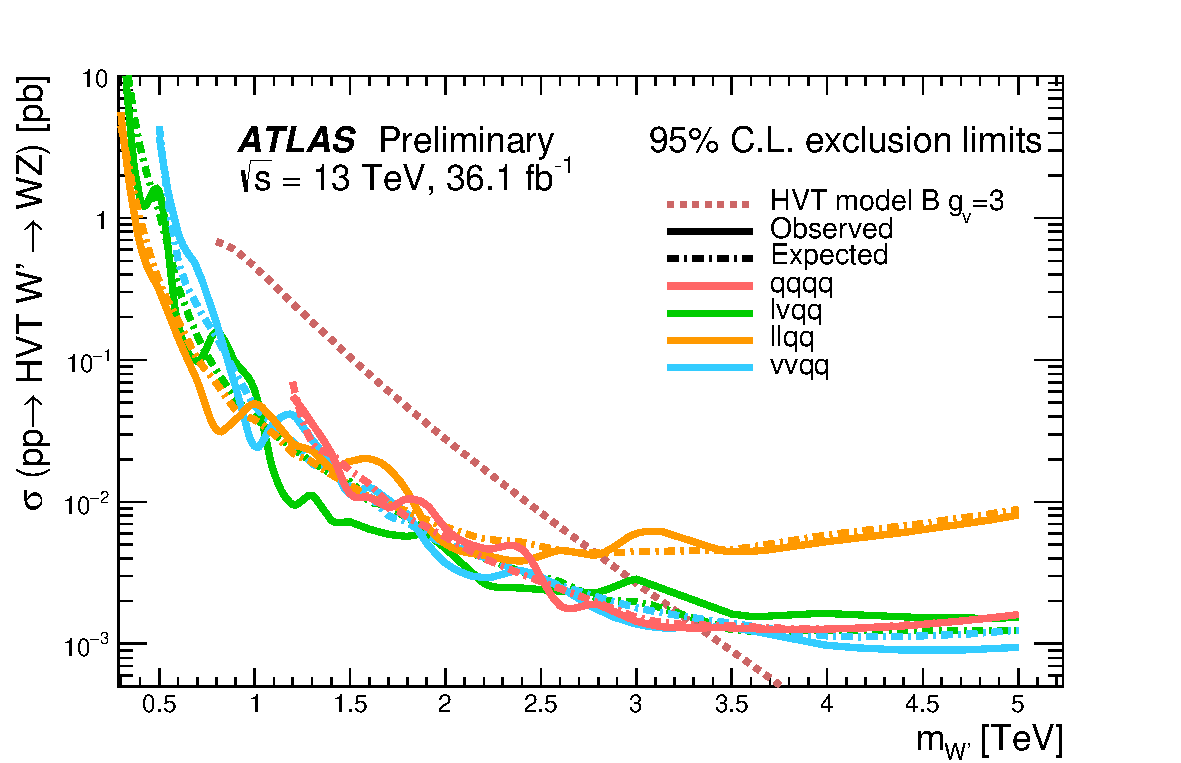
\includegraphics[width=.495\textwidth]{figures/ATLAS_Diboson_Summary.pdf}
  \caption{The observed and expected limits on the product of the cross-section and branching fraction $\sigma \mathcal{B} (W' \rightarrow WZ)$ for a spin-1 $W'$, as a function of the reconstructed mass of the diboson resonance. The dark red dotted line shows the theoretical predictions for the HVT model B.~\cite{ATLASPublicResults}}
  \label{fig:theory_ATLAS_Diboson_Summary}
\end{figure}

\begin{figure}[!htb]
  \centering
    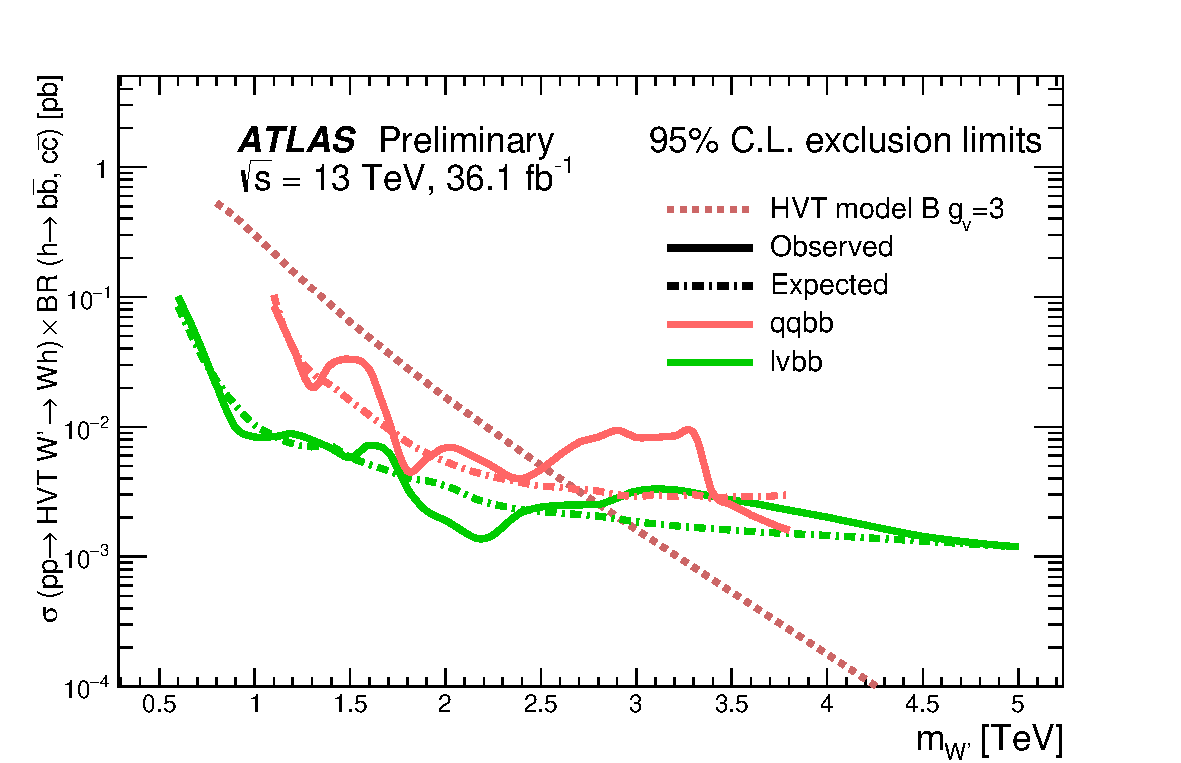
\includegraphics[width=.495\textwidth]{figures/ATLAS_Diboson_Summary_VH.pdf}%
    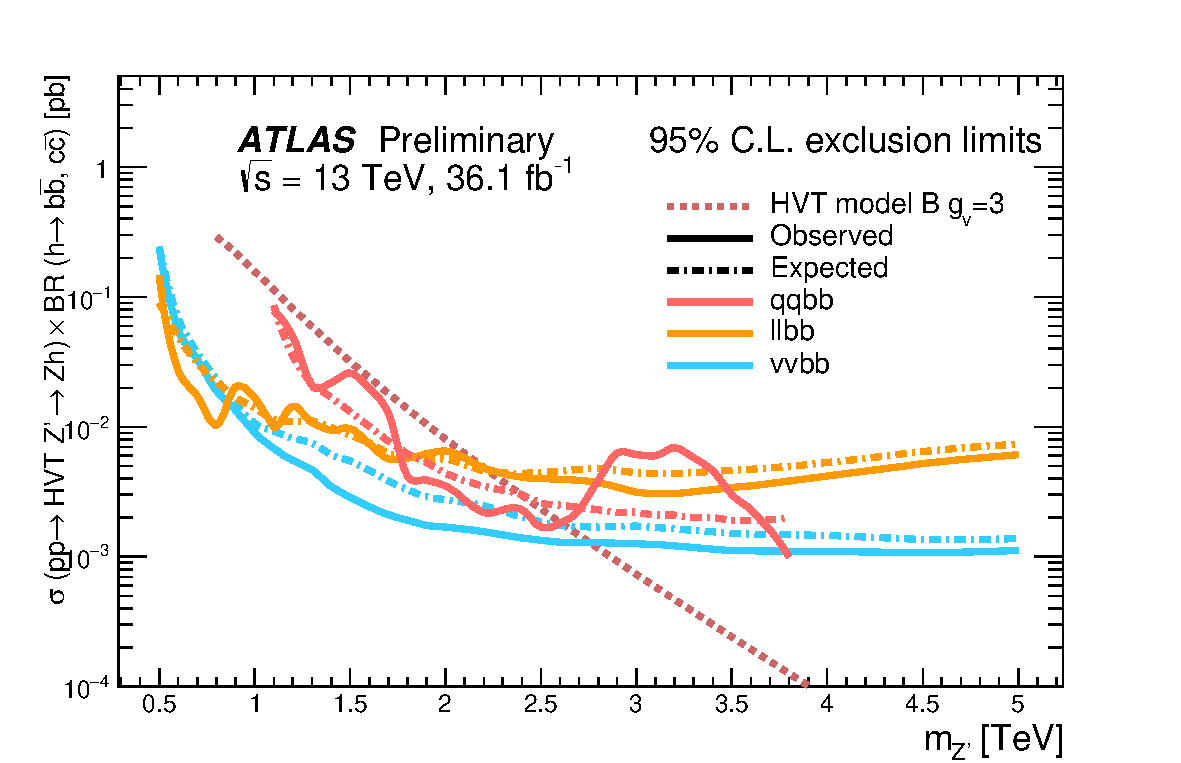
\includegraphics[width=.495\textwidth]{figures/ATLAS_Diboson_Summary_VV_ZP.pdf}
  \caption{The observed and expected limits on the product of the cross-section and branching fraction $\sigma \mathcal{B} (W' \rightarrow WH)$ for a spin-1 $W'$ (left) and $\sigma \mathcal{B} (Z' \rightarrow ZH)$ for a spin-1 $Z'$ (right), as a function of the reconstructed mass of the diboson resonance. The dark red dotted lines show the theoretical predictions for the HVT model B.~\cite{ATLASPublicResults}}
  \label{fig:theory_ATLAS_Diboson_Summary_VH}
\end{figure}
%Data collected by ATLAS and CMS experiments are used to set limits on the HVT resonance masses and coupling parameters. Experimental results, both from Run 1 LHC data (at a center-of-mass energy of 8 TeV) brought to the following conclusions. A weakly coupled resonance, in the context of benchmark model A ($g_V = 1$) was excluded up to 3 TeV by Run 1 data. By looking at parton luminosities in fig.\ref{fig:HVT_DY_partolumi}, in data produced by LHC proton-proton collision at 14 TeV, collected for an integrated luminosity of 300 $\mbox{fb}^{-1}$, sensitivity was expected to increase up to $m_V \approx 6$ TeV. A strongly coupled resonance, in the context of benchmark model B ($g_V = 3$) is excluded up to 2 TeV by Run 1 data. Data produced by LHC at 14 TeV should have increased the sensitivity up to $m_V \approx 3-4$ TeV.\\
%No evidence of HVT resonances has been observed so far. ~\cite{CMS-PAS-B2G-16-007,Aad:2015ipg}. The most stringent limits have been set by LHC data collected in 2016 during Run 2 proton-proton collisions, performed at a center-of-mass energy of 13 TeV.

\clearpage
\section{Warped extra-dimension}
\label{sec:theory_WED}
The Randall-Sundrum model~\cite{Randall:1999ee,Randall:1999vf} (RS1) proposes the introduction of one additional warped dimension in order to solve the hierarchy problem. The metric of the 5-dimensional space (a slice of $AdS_5$) generates an exponential hierarchy between the electroweak and Planck scales, associated respectively to the TeV three-brane, where the SM particles are confined, and the Planck three-brane. As a consequence of the new geometry, spin-2 massive gravitons are predicted to exist.\\
The bulk extension of the Randall-Sundrum model~\cite{Agashe:2007zd,Fitzpatrick:2007qr} states that the SM fields can propagate in the extra-dimension. Light fermions are near the Planck brane, heavy fermions are close to the TeV brane, while the Higgs sector is confined in the TeV brane. Higgs couplings to the heavy fermions are therefore expected to be stronger: this naturally arising hierarchy of the masses of the SM fields gives a solution to the flavour problem. In this scenario, the fermionic decays of the bulk gravitons are suppressed, while the bosonic decays are preferred.

\subsection{Randall-Sundrum original model (RS1)}
\label{sec:RS1}
The existence of additional $n$-dimensions implies that the effective Planck scale observed in 4-dimensions, $M_{PL} = 1.2209 10^{19}$ GeV, is related to the fundamental 4+$n$-dimensional Planck scale, $M$, via the geometry. %$M$ is expected to be of the order of the reduced $\overline{M}_{PL} = M_{PL}/2 \pi$. 
If the 4-dimensional and the $n$ additional metrics are factorizable, the reduced Planck scale $\overline{M}_{PL} = M_{PL}/2 \pi$ can be seen as the product of $M$ and the volume of the compact space $V_n$:

\begin{equation}
\overline{M}_{PL}^2 = V_n M^{2+n}.
\label{eq:theory_planck_mass}
\end{equation}

\noindent If $M \sim$ TeV, this implies that $V_n$ must be very large, hence the compactification scale $\mu~\sim~1/V_n^{1/n}$ is necessarily small (eV -- MeV for n=2 -- 7).  Given the smallness of $\mu$ when compared to the electroweak scale, the effects of the $n$ extra-dimensions should be evident in SM processes. Since they are not observed, SM particles are assumed to be confined in a 4-dimensional space, the TeV three-brane, while only gravity is allowed to propagate into the 4+$n$-dimensional space, the bulk. This mechanism solves the hierarchy of the Higgs scale, but on the other hand it introduces a new hierarchy between $\mu$ and $M$.\\
In the Randall-Sundrum model~\cite{Randall:1999ee,Randall:1999vf}, only one additional dimension is added. The geometry of the 5-dimensional bulk is non-factorizable, and it is a slice of $AdS_5$ spacetime.\footnote{An $n$-dimensional anti-de Sitter space ($AdS_n$) is a maximally simmetric Lorentzian mainfold, that solves the Einstein equation with a negative curvature (negative cosmological constant).} The 4-dimensional metric is multiplied by an exponential function of the fifth dimension (the ``warp'' factor):

\begin{equation}
ds^2 = e^{-2 k r_c \varphi} \eta_{\mu \nu} dx^{\mu} dx^{\nu} + r_c^2 d{\varphi}^2;
\label{eq:theory_metric}
\end{equation}

\noindent $x^{\mu}$ are the usual 4-dimensional coordinates, $\eta_{\mu \nu} = \text{diag}(-1, 1, 1, 1)$ is the Minkowski metric, $k$ is a scale of order of $\overline{M}_{PL}$, $\varphi$ is the coordinate of the extra-dimension, $0 < |\varphi| < \pi$, and $r_c$ is the compactification radius of this finite interval. 4-dimensional mass scales are obtained by multiplying the bulk masses by $e^{-2 k r_c \varphi}$: given the exponential form of the warp factor, a small $r_c$ suffices for generating a large hierarchy between Planck and Higgs scales.\\
Two 4-dimensional three-branes are located at the boundaries of the fifth dimension: the visible brane at $\varphi = \pi$; the hidden brane at $\varphi = 0$, and their metrics are obtained starting from the bulk 5-dimensional metric $G_{MN}$, where $M,N = \mu, \varphi$:

\begin{equation}
\begin{split}
 & g_{\mu \nu}^{\text{vis}} (x^{\mu}) = G_{\mu \nu} \left( x^{\mu}, \varphi = \pi \right),\\
 & g_{\mu \nu}^{\text{hid}} (x^{\mu}) = G_{\mu \nu} \left( x^{\mu}, \varphi = 0 \right).\\
\end{split}
\label{eq:theory_brane_metrics}
\end{equation}

\noindent The classical action is given by:

\begin{equation}
\begin{split}
 & S = S_{\text{gravity}} + S_{\text{vis}} + S_{\text{hid}},\\
 & S_{\text{gravity}} = \int d^4x \int_{-\pi}^{+\pi} d\varphi \sqrt{-G} \left( -\Lambda + 2 M^3 \mathcal{R} \right),\\
 & S_{\text{vis}} = \int d^4x \sqrt{-g_{\text{vis}}} \left( \mathcal{L_{\text{vis}}} -V_{\text{vis}} \right),\\
 & S_{\text{hid}} = \int d^4x \sqrt{-g_{\text{hid}}} \left( \mathcal{L_{\text{hid}}} -V_{\text{hid}} \right),\\
\end{split}
\label{eq:theory_classical_action}
\end{equation}

\noindent where $G$ ($g$) is the trace of the $G_{MN}$ ($g_{\mu \nu}$) metric, $\Lambda$ is the cosmological constant in the bulk, $\mathcal{R}$ is the 5-dimensional Ricci scalar, $\mathcal{L}$ and $V$ are the lagrangian and the vacuum energy of the hidden and visible branes.\\
A 5-dimensional metric that preserves the 4-dimensional Poincar\'e invariance has the form:

\begin{equation}
ds^2 = e^{-2 \sigma(\varphi)} \eta_{\mu \nu} dx^{\mu} dx^{\nu} + r_c^2 d{\varphi}^2.
\label{eq:theory_poincare_metric}
\end{equation}

\noindent The Poincar\'e invariance guarantees that $r_c$ does not depend on $x^{\mu}$. Given~\ref{eq:theory_poincare_metric}, the solution of the 5-dimensional Einstein's equations simplifies into:

\begin{equation}
\sigma = r_c \left| \varphi \right| \sqrt{\frac{- \Lambda}{24 M^3}}.
\label{eq:theory_einstein_solution}
\end{equation}


\noindent Furthermore, the Poincar\'e invariance imposes constraints to the vacuum energies and cosmological constant:

\begin{equation}
\begin{split}
 & V_{\text{hid}} = - V_{\text{vis}} = 24 M^3 k \\
 & \Lambda = -24 M^3 k^2.\\
\end{split}
\label{eq:theory_vacuum_energies}
\end{equation}

\noindent The final 5-dimensional metric is then:

\begin{equation}
ds^2 = e^{-2 k r_c \left| \varphi \right|} \eta_{\mu \nu} dx^{\mu} dx^{\nu} + r_c^2 d{\varphi}^2.
\label{eq:theory_metric_solution}
\end{equation}

\noindent A small $r_c$ is considered, so the effects of the fifth dimension on the 4-dimensional spacetime can't be appreciated. A 4-dimensional effective field theory approach is therefore motivated, and its mass parameters are related to the bulk parameters, $M$, $k$ and $r_c$. In the Randall-Sundrum model, the SM matter fields are confined in the TeV brane.\\
The massless gravitons, the mediators of the gravitational interaction in the effective field theory, are the zero modes ($h_{\mu \nu}$) of the quantum fluctuations of the classical solution (~\ref{eq:theory_metric_solution}):

\begin{equation}
ds^2 = e^{-2 k T(x) \left| \varphi \right|} \left( \eta_{\mu \nu} + h_{\mu \nu}(x) \right) dx^{\mu} dx^{\nu} + T^2(x) d{\varphi}^2,
\label{eq:theory_metric_perturbation}
\end{equation}

\noindent where the usual Minkowski metric has been replaced by $\overline{g}_{\mu \nu} (x) = \eta_{\mu \nu} + h_{\mu \nu}$; $h_{\mu \nu}$ are the tensor fluctuations around the Minkowski space, and represent both the physical graviton in 4-dimensions and the massless mode of the Kaluza-Klein decomposition of the bulk metric. $r_c$ is the vacuum expectation value of $T(x)$.\\
By substituting eq.~\ref{eq:theory_metric_perturbation} in the classical action~\ref{eq:theory_classical_action}, an effective action can be extracted, and in particular the curvature term holds:

\begin{equation}
S_{\text{eff}} \sim \int d^4 x \int_{-\pi}^{+\pi} d \varphi 2 M^3 r_c e^{-2 k r_c \left| \varphi \right|} \overline{\mathcal{R}} \sqrt{-\overline{g}},
\label{eq:theory_effective_action}
\end{equation}

\noindent where $\overline{g}$ is the trace of $\overline{g}_{\mu \nu}$ and $\overline{\mathcal{R}}$ is the 4-dimensional Ricci scalar of $\overline{g}_{\mu \nu}$ metric. In this effective 4-dimensional action, the $\varphi$ dependence can be integrated out, and the 4-dimensional Planck mass can be calculated:

\begin{equation}
\overline{M}_{PL}^2 = M^3 r_c \int_{-\pi}^{+\pi} d \varphi e^{-2 k r_c \left| \varphi \right|} = \frac{M^3}{k} \left( 1 - e^{-2 k r_c \pi} \right).
\label{eq:theory_effective_planck_mass}
\end{equation}

\noindent It can be shown~\cite{Randall:1999ee} that a field with a fundamental mass parameter $m_0$ in the bulk manifests in the visible three-brane with a physical mass $m$:

\begin{equation}
m = e^{- k r_c \pi} m_0.
\label{eq:theory_effective_masses}
\end{equation}

\noindent Scales $m \sim$ TeV are generated from $m_0 \sim \overline{M}_{PL}$ if $e^{k r_c \pi} \sim 10^{15}$. This relation stands still when Higgs field is introduced and confined in the visible three-brane:

\begin{equation}
v = e^{- k r_c \pi} v_0,
\label{eq:theory_effective_Higgs_vev}
\end{equation}

\noindent where $v$ is the Higgs vacuum expectation value in the TeV brane and $v_0$ is the 5-dimensional Higgs v.e.v.\\
The hierarchy problem is then solved by the exponential warp factor. The weakness of gravity in the TeV three-brane is motivated by the small overlap with the graviton wave function.\\
In order to calculate the mass spectrum of the graviton in the TeV brane, the tensor fluctuations of the Minkowski metric are expanded into a Kaluza-Klein (KK) tower $h_{\mu \nu}^{(n)}$:

\begin{equation}
h_{\mu \nu}(x, \varphi) = \sum_{n=0}^{\infty} h_{\mu \nu}^{(n)}(x) \frac{\chi^{(n)}(\varphi)}{\sqrt{r_c}}.
\label{eq:theory_RS_KK_tower}
\end{equation}

\noindent Once a suitable gauge is chosen, \textit{i.e.} $\eta^{\mu \nu} \partial_{\mu} h_{\nu \alpha}^{(n)} = \eta^{\mu \nu} h_{\mu \nu}^{(n)} = 0$, the equation of motion of $h_{\mu \nu}^{(n)}$ becomes the Klein-Gordon relation, where $m_n^G \geq 0$:

\begin{equation}
\left( \eta^{\mu \nu} \partial_{\mu} \partial_{\nu} - (m_n^G)^2 \right) h_{\mu \nu}^{(n)}(x)= 0.
\label{eq:theory_RS_KK_KleinGordon}
\end{equation}

\noindent By substituting eq.~\ref{eq:theory_RS_KK_tower} into Einstein's equation, the solutions for $\chi^{(n)}(\varphi)$ (commonly called ``profiles'') are~\cite{Davoudiasl:1999jd,Gherghetta:2000qt}:

\begin{equation}
\chi^{(n)}(\varphi) = \frac{e^{2 \sigma}}{N} \left[ J_2(z_n^G) + \alpha_n Y_2(z_n^G) \right],
\label{eq:theory_RS_KK_tower_profile}
\end{equation}

\noindent where $J_2$ and $Y_2$ are second order Bessel functions, $N$ is the normalization of the wavefunction, $\alpha_n$ are coefficients and $z_n^G = m_n^G e^{\sigma(\varphi)}/k$. $m_n^G$ is the mass of the $n$-mode, and it depends on the roots of the Bessel functions $z_n^G = \left( 3.83, 7.02, 10.17, 13.32, ... \right)$. In the limit $m_n^G/k \ll 1$ and $e^{k r_c \pi} \gg 1$:

\begin{equation}
m_n^G = k z_n^G(\pi) e^{-k r_c \pi}.
\label{eq:theory_RS_KK_tower_mass}
\end{equation}

\noindent The interactions between the graviton KK modes and the matter fields in the TeV brane can be derived from the 4-dimensional effective Lagrangian, once $h_{\mu \nu}$ is replaced by its KK decomposition:

\begin{equation}
\mathcal{L} = - \frac{1}{\overline{M}_{PL}} T^{\mu \nu}(x) h_{\mu \nu}^{(0)} - \frac{1}{e^{-k r_c \pi} \overline{M}_{PL}} T^{\mu \nu}(x) \sum_{n=1}^{\infty}h_{\mu \nu}^{(n)}(x);
\label{eq:theory_RS_KK_lagrangian}
\end{equation}

\noindent $T^{\mu \nu}$ is the space energy-momentum tensor of the matter fields. The zero mode of the gravitons coupling is $1/\overline{M}_{PL}$, while higher order KK modes couplings to all SM fields are suppressed by $e^{-k r_c \pi} \overline{M}_{PL}$, that is of the order of the TeV scale. Spin-2 KK masses and couplings are hence determined by the TeV scale, or, equivalently, KK gravitons are close to the TeV brane. This implies that KK gravitons can be produced via $q \bar{q}$ or gluon fusion, and that a leptonic decay of the resonance could represent a very clear signal signature.

\subsection{Bulk extension of RS1: graviton production and decays}
\label{sec:BG}
An extension of the original RS1 formulation has been proposed. It states that the usual SM fields are no longer confined in the TeV brane, but they are the zero modes of the corresponding 5-dimensional SM fields. If first and second generation fermions are close to the Planck brane, contribution to flavour changing neutral currents by higher-dimensional operators are suppressed. These contributions are excluded by electroweak precision tests, but they were not prevented in original RS1. The second motivation behind the choice is, as mentioned previously, the naturally arising flavour hierarchy: first and second generation quarks have small Yukawa couplings to the Higgs sector, confined in the TeV brane, while top quark and bosons have stronger Yukawa couplings.\\
In this picture, couplings between higher-order KK gravitons and light fermions are strongly suppressed, resulting into a negligible KK gravitons production via $q \bar{q}$, whilst gluon fusion production becomes dominant. KK gravitons decays into top quarks and Higgs bosons are dominant, given that both their profiles are near the TeV brane, while leptonic decays are negligible. Via the equivalence theorem, the Goldstone bosons are equivalent to the longitudinally polarized weak bosons, $W_L^{\pm}$ and $Z_L$, that have profiles close to the TeV brane. Decays of KK gravitons into weak dibosons (and production in VBF) are comparable to di-top and di-Higgs decays.\\

\noindent The KK decomposition and the KK mass spectrum of the graviton have already been presented in sec.~\ref{sec:RS1}. The KK decomposition of a massless 5-dimensional gauge field $A_M(x, \varphi)$ is similarly performed~\cite{Davoudiasl:2000wi}:

\begin{equation}
A_{\mu}(x, \varphi) = \sum_{n=0}^{\infty} A_{\mu}^{(n)}(x) \frac{\chi^{(n)}_A(\varphi)}{\sqrt{r_c}}.
\label{eq:theory_gauge_KK_tower}
\end{equation}

\noindent The profiles for the gauge fields are:

\begin{equation}
\chi^{(n)}_A(\varphi) = \frac{e^{\sigma}}{N_A} \left[ J_1(z_n^A) + \alpha_n^A Y_1(z_n^A) \right],
\label{eq:theory_gauge_KK_tower_profile}
\end{equation}

\noindent where $J_1$ and $Y_1$ are first order Bessel functions. Similarly to eq.~\ref{eq:theory_RS_KK_tower_mass}, the mass spectrum of the gauge field is:

\begin{equation}
m_n^A = k z_n^A(\pi) e^{-k r_c \pi};
\label{eq:theory_RS_KK_tower_mass}
\end{equation}

\noindent the first roots of the Bessel functions are $z_n^A = \left( 2.45, 5.57, 8.70, 11.84, ... \right)$.

\noindent The Lagrangian expressing the interaction between the $m$ and $n$ modes of the bulk field $F$ to the $q$ KK gravitons mode $G$ is~\cite{Davoudiasl:2000wi}:

\begin{equation}
\mathcal{L}_{G-F} = \sum_{m,n,q} C_{mnq}^{FFG} \frac{1}{\overline{M}_{PL}} \eta^{\mu \alpha} \eta^{\nu \beta} h_{\alpha \beta}^{(q)} (x) T_{\mu \nu}^{(m,n)}(x),
\label{eq:theory_lagrangian_bulk_KK}
\end{equation}

\noindent $C_{mnq}^{FFG}$ is the overlap integral of the profiles:

\begin{equation}
C_{mnq}^{FFG} = \int \frac{d \varphi}{\sqrt{k}} e^{t \sigma} \frac{\chi_F^{(m)} \chi_F^{(n)} \chi_G^{(q)}}{\sqrt{r_c}};
\label{eq:theory_overlap_integral}
\end{equation}

\noindent $t$ depends on the type of field considered.\\
The coupling between gluons and the $q$ KK graviton mode is given by:

\begin{equation}
C_{00q}^{AAG} = e^{k \pi r_c} \frac{2 \left[ 1 - J_0 (x_q^G)\right]}{k \pi r_c \left(x_q^G \right)^2 \left| J_2 (x_q^G)\right|}.
\label{eq:theory_overlap_integral_ggG}
\end{equation}

\noindent Once eq.~\ref{eq:theory_overlap_integral_ggG} is put in eq.~\ref{eq:theory_lagrangian_bulk_KK}, the most significant partial decay widths into the $q$ KK graviton mode are:

\begin{equation}
\begin{split}
 & \Gamma \left(G \rightarrow t_R \bar{t}_R \right) \sim N_c \frac{ \left[ \tilde{k} x_q^G \right]^2 m_q^G}{320 \pi}, \\
 & \Gamma \left(G \rightarrow h h \right) \sim \frac{\left[ \tilde{k} x_q^G \right]^2 m_q^G}{960 \pi}, \\
 & \Gamma \left(G \rightarrow W^+_L W^-_L \right) \sim \frac{\left[ \tilde{k} x_q^G \right]^2 m_q^G}{480 \pi}, \\
 & \Gamma \left(G \rightarrow Z_L Z_L \right) \sim \frac{\left[ \tilde{k} x_q^G \right]^2 m_q^G}{960 \pi}, \\
\end{split}
\label{eq:theory_bulk_KK_partial_decay_widths}
\end{equation}

\noindent where $\tilde{k} = k/\overline{M}_{PL}$; the total decay width is:

\begin{equation}
\Gamma_G = \frac{13 \left[ \tilde{k} x_q^G \right]^2 m_q^G}{960 \pi}.
\label{eq:theory_bulk_KK_total_decay_width}
\end{equation}

\noindent Calculations, so far, have been performed considering $M \sim \overline{M}_{PL}$ and $k < M$, hypotheses under which the solution for the bulk metric (eq.~\ref{eq:theory_metric_solution}) is valid. Hence, $\tilde{k} = k / \overline{M}_{PL} \leq 1$ is taken as a reference interval. This has also phenomenological consequences on the width of the resonance, as stated in eq.~\ref{eq:theory_bulk_KK_total_decay_width}. The total decay width of the lightest KK graviton mode, compared to its mass, is shown as a function of $\tilde{k}$ in fig.~\ref{fig:theory_grav_width_vs_ktilda}~\cite{Oliveira:2014kla}. At $\tilde{k} = 1$, in the bulk scenario, the KK graviton width is expected to be few \% of its mass, up to 4 TeV (dotted red curve). The narrow width approximation holds, hence the resonance properties can be probed at the peak, neglecting the effects in the tails of the mass distribution.

\begin{figure}[!htb]
  \centering
    \includegraphics[width=.495\textwidth]{figures/1404_0102_fig.pdf}
  \caption{Width of the KK gravitons, in units of the mass of the resonance, as a function of the curvature parameter $\tilde{k}$. The red curves represent the bulk extension of RS1 original model for different mass hypotheses (from 500 GeV up to 4 TeV).~\cite{Oliveira:2014kla}}
  \label{fig:theory_grav_width_vs_ktilda}
\end{figure}

\noindent The total cross-section of a bulk graviton, produced at the LHC in proton-proton interactions via gluon fusion (displayed in fig.~\ref{fig:theory_KK_gg_prod}), decaying into a couple of vector bosons (for the purpose of this thesis, a final state with two longitudinally polarized $Z$ bosons is considered) is expressed as a function of the parton level cross-section $\hat{\sigma}$, the gluon parton distribution functions $f_q$, the momentum transfer $Q^2 \sim (m_q^G)^2$ and the center-of-mass energy $s$:

\begin{equation}
\sigma(pp \rightarrow ZZ) = \int dx_1 dx_2 f_g(x_1,Q^2) f_g(x_2, Q^2) \hat{\sigma}(x_1 x_2 s).
\label{eq:theory_cross_section_bulk}
\end{equation}

\noindent The differential parton level cross-section, averaged over colors and initial spin states, is (hatted quantities are calculated in the center-of-mass frame):

\begin{equation}
\frac{d \hat{\sigma}(gg \rightarrow ZZ)}{d \cos{\hat{\theta}}} \approx \frac{ \left| \mathcal{M}_{+-00}\right|^2}{1024 \pi \hat{s}},
\label{eq:theory_parton_level_cross_section_bulk}
\end{equation}

\noindent where $\left| \mathcal{M}_{+-00}\right|$ is the matrix element of the dominant contribution in $gg \rightarrow VV$ process ($\Gamma_G$ is defined in eq.~\ref{eq:theory_bulk_KK_total_decay_width}, $a$, $b$ are colour factors):

\begin{equation}
\mathcal{M}_{+-00} (g^a g^b \rightarrow VV) = -C_{00q}^{AAG} e^{-k \pi r_c} \left( \frac{x^G_n \tilde{k}}{m_n^G}\right)^2 \sum_n \frac{\delta_{ab} \mathcal{A}_{+-00}}{\hat{s} - {m_n^G}^2 +i \Gamma_G m_n^G}.
\label{eq:theory_KK_matrix_elements}
\end{equation}

\noindent The relevant amplitudes taken account in the matrix element calculation are~\cite{Agashe:2007zd}:

\begin{equation}
%\begin{split}
\mathcal{A}_{+-00} = \mathcal{A}_{-+00} = \frac{\left( 1 - 1/\beta_Z^2 \right) \left( \beta_Z^2 -2\right) \left[ (\hat{t} - \hat{u})^2 - \beta_Z^2\hat{s}^2 \right] \hat{s} }{8 M_Z^2},
%\end{split}
\label{eq:theory_KK_amplitudes}
\end{equation}

\noindent where $\beta_Z^2 = 1- 4M_Z^2/\hat{s}$ and $M_Z$ is the mass of the $Z$ boson.

\begin{figure}[!htb]
  \centering
\feynmandiagram [horizontal=a to b] {
  i1 [particle=\(g\)] -- [gluon] a -- [gluon] i2 [particle=\(g' \)],
  a -- [red!80!black, boson, edge label=\(G\), very thick] b,
  f1 [particle=\(Z\)] -- [boson] b -- [boson] f2 [particle=\(Z\)],
};
\caption{Gluon fusion production mechanism for a KK graviton that decays into a couple of $Z$ bosons.}
\label{fig:theory_KK_gg_prod}
\end{figure}

%\newpage
\subsection{Search for KK bulk gravitons at LHC}
\label{sec:theory_KK_limits_LHC}
No evidence of spin-2 bulk graviton resonances has been observed so far at the LHC experiments. Data collected by the ATLAS and CMS detectors are used to set limits on the graviton masses, generally considering different curvature parameter $\tilde{k}$ hypotheses, once assured the narrow width approximation is still valid (up to $\tilde{k} \sim 1$). The most stringent limits have been set with Run 2 data.

\vspace*{1\baselineskip}

\noindent Many results of the diboson searches performed at CMS and already presented in sec.~\ref{sec:theory_HVT_limits_LHC} are interpreted in the context of the bulk graviton models, together with the additional final states $ZZ \rightarrow \ell \bar{\ell} \nu \bar{\nu}$~\cite{CMS-PAS-B2G-16-023} and $HH \rightarrow b\bar{b} b \bar{b}$~\cite{CMS-PAS-B2G-16-026}. The most interesting limit is provided by the search for $ZZ \rightarrow \ell \bar{\ell} \nu \bar{\nu}$ resonances~\cite{CMS-PAS-B2G-16-023}, that, under the hypothesis $\tilde{k} = 0.5$, excludes a spin-2 bulk graviton with a mass lower than 800 GeV (fig.~\ref{fig:theory_B2G-16-023}).

\begin{figure}[!htb]
  \centering
    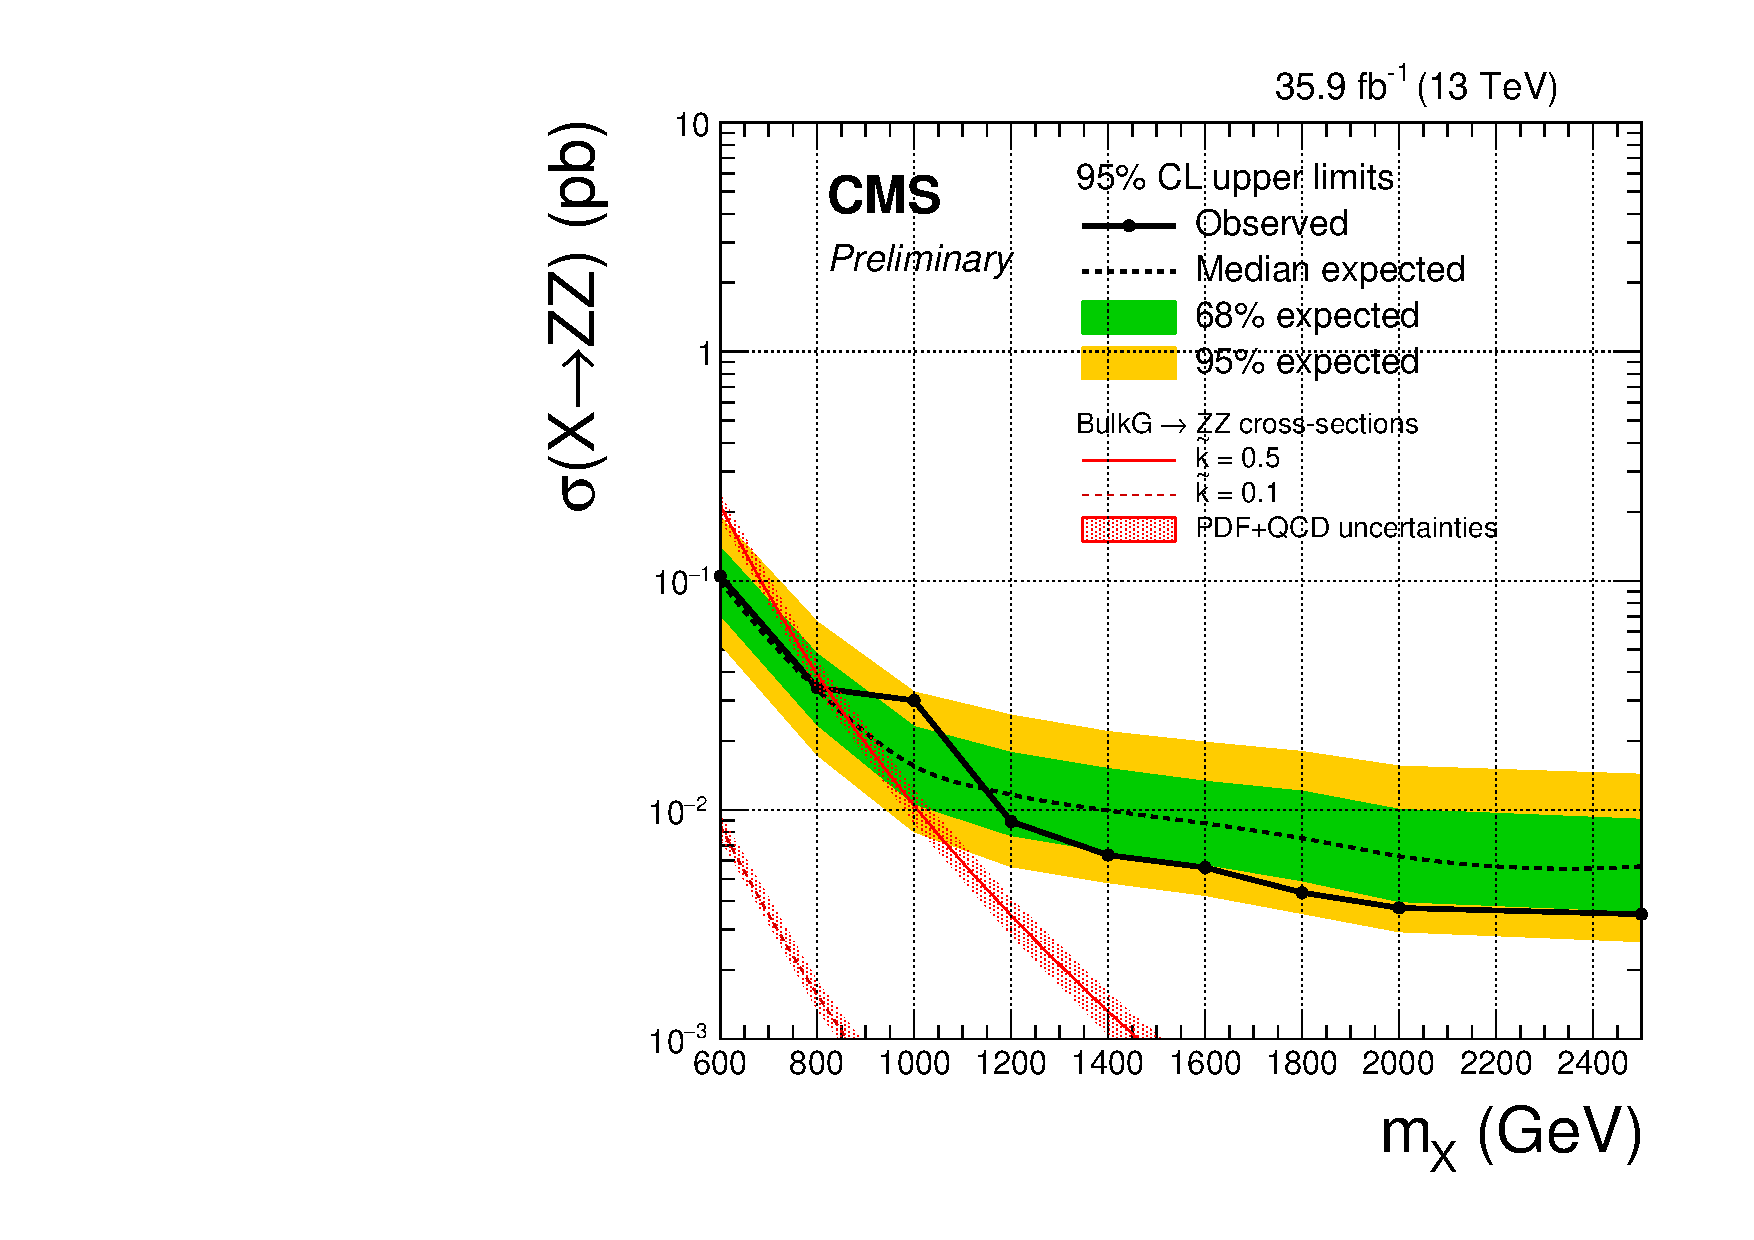
\includegraphics[width=.495\textwidth]{figures/B2G-16-023/Figure_005.pdf}
  \caption{The observed and expected limits, with 68\% and 95\% uncertainty bands, on the product of the cross-section and branching fraction $\sigma \mathcal{B} (G \rightarrow ZZ)$ for a spin-2 bulk graviton, as a function of the reconstructed mass of the diboson resonance. The coloured lines show the theoretical predictions for $\tilde{k}=0.1$ and $0.5$.~\cite{CMS-PAS-B2G-16-023}}
  \label{fig:theory_B2G-16-023}
\end{figure}

\vspace*{1\baselineskip}

%Revision
%
%\noindent The results (or preliminary results) on bulk graviton searches in diboson final states, performed with 2016 data and published by the CMS Collaboration so far, are summarized in fig.~\ref{fig:theory_CMS_Diboson_Summary_graviton}. The dark orange curve and the pink curve correspond to two possible final states included the $(ZZ, WW) \rightarrow q\bar{q}q\bar{q}$ analysis~\cite{Sirunyan:2017acf,bib:CMS-PAS-B2G-17-001}; the light blue curve corresponds to the $ZZ \rightarrow \ell \ell \nu \nu$ analysis~\cite{CMS-PAS-B2G-16-023}; the green curve corresponds to the $HH \rightarrow b\bar{b} b \bar{b}$ analysis~\cite{CMS-PAS-B2G-16-026}; the light orange curve corresponds to the analysis discussed in this thesis~\cite{CMS-PAS-B2G-17-005}.
\noindent The results (or preliminary results) on bulk graviton searches in diboson final states, performed with 2016 data and published by the CMS Collaboration so far, are summarized in fig.~\ref{fig:theory_CMS_Diboson_Summary_graviton}.  

\begin{figure}[!htb]
  \centering
    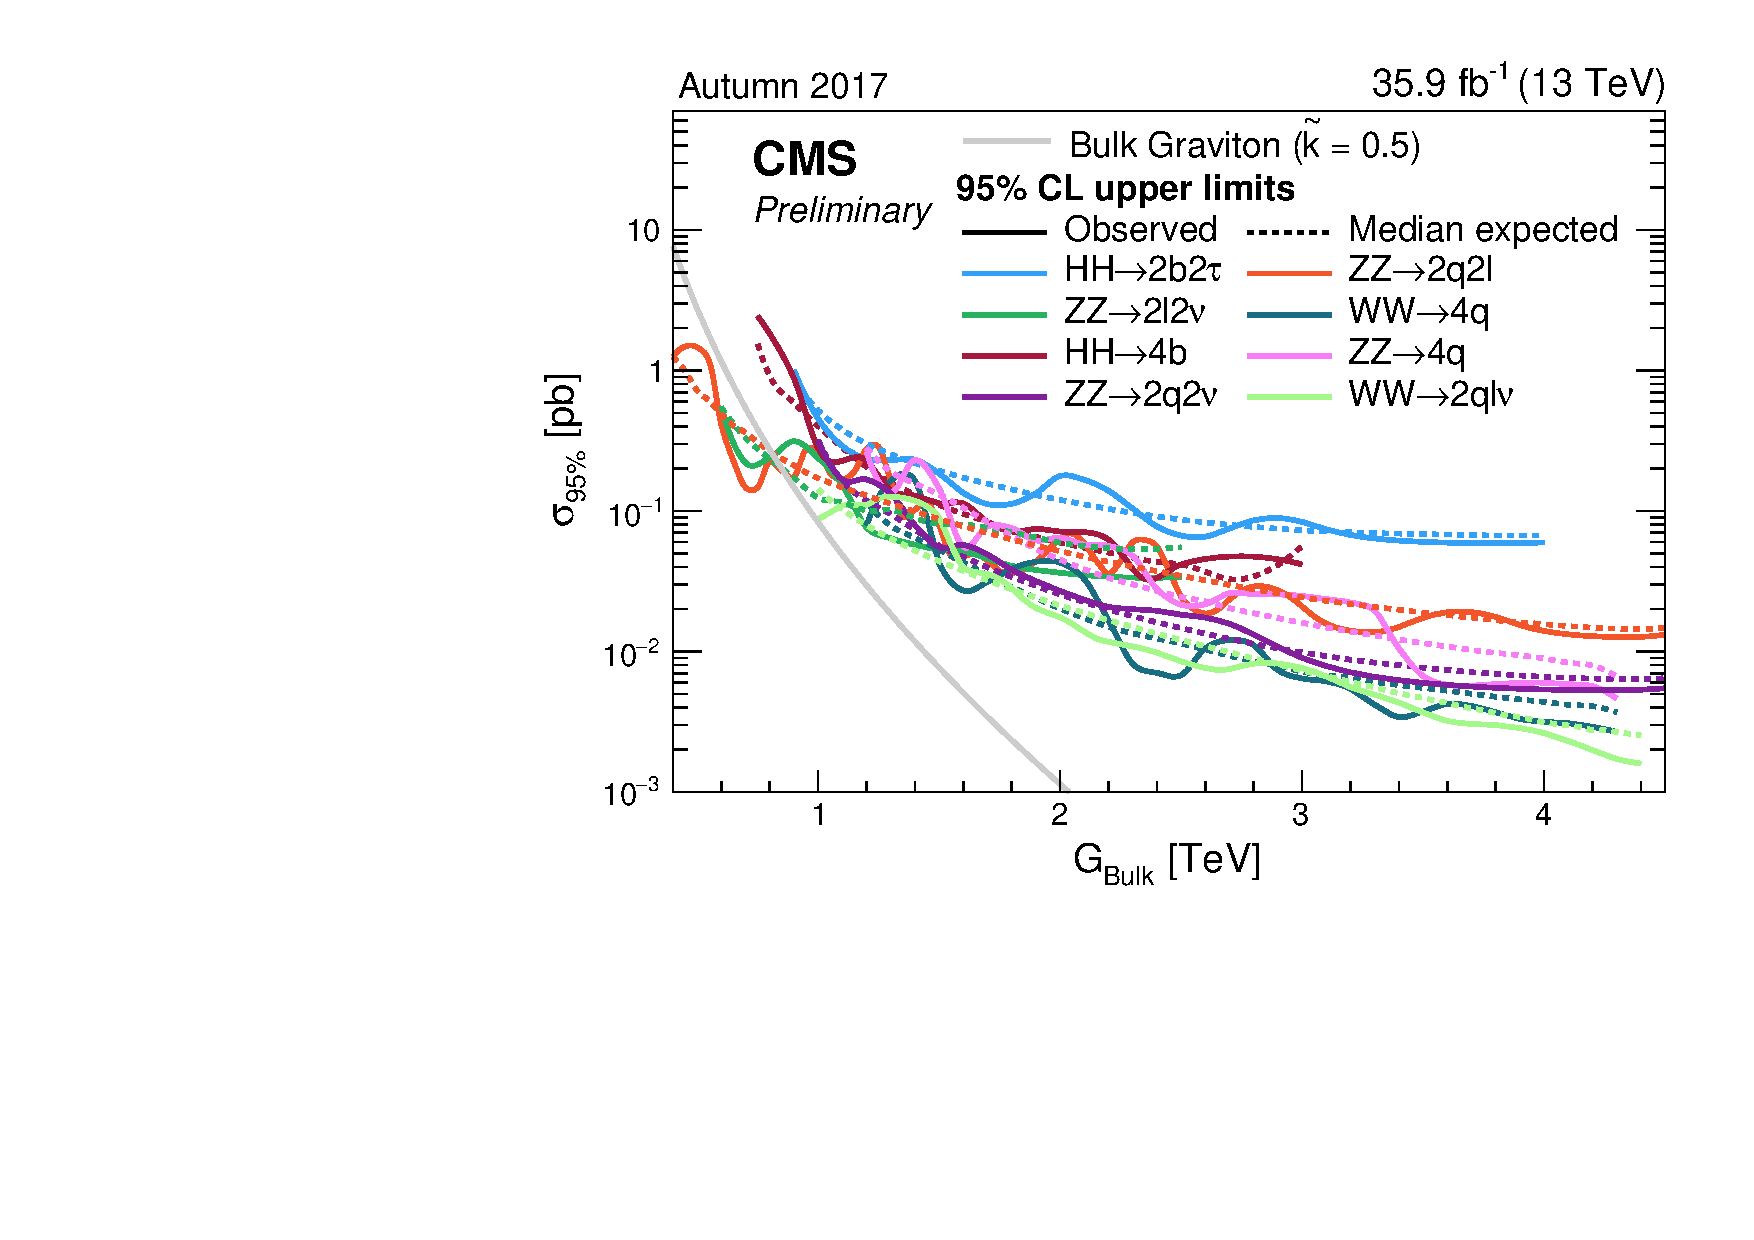
\includegraphics[width=.495\textwidth]{figures/Autumn2017/combiLimitsBulkG_BulkG.pdf}
  \caption{The observed and expected limits on the product of the cross-section and branching fraction $\sigma \mathcal{B} (G \rightarrow (WW, ZZ))$ for a spin-2 bulk graviton, as a function of the reconstructed mass of the diboson resonance.~\cite{CMSDibPublicResults} The gray line shows the theoretical prediction for the bulk graviton model, once assumed a curvature parameter $\tilde{k}=0.5$. The light blue curve corresponds to the $HH \rightarrow b \bar{b} \tau^+ \tau^-, (WH, ZH) \rightarrow q \bar{q} \tau^+ \tau^-$ analysis~\cite{CMS-PAS-B2G-17-006}; the bright green curve corresponds to the $ZZ \rightarrow \ell \ell \nu \nu$ analysis~\cite{CMS-PAS-B2G-16-023}; the dark red curve corresponds to the $HH \rightarrow b\bar{b} b \bar{b}$ analysis~\cite{CMS-PAS-B2G-16-026}; the dark orange curve corresponds to the $ZW, ZZ \rightarrow \ell \bar{\ell} q\bar{q}$ analysis~\cite{CMS-PAS-B2G-17-013}; the dark green curve and the pink curve correspond to two possible final states included in the $(WZ, WW) \rightarrow q\bar{q}q\bar{q}$ analysis~\cite{Sirunyan:2017acf,bib:CMS-PAS-B2G-17-001}; the light green curve corresponds to the $WZ, WW \rightarrow \ell \nu q \bar{q}$ analysis~\cite{CMS-PAS-B2G-16-029}; finally, the violet curve corresponds to the analysis discussed in this thesis~\cite{CMS-PAS-B2G-17-005}.}
  \label{fig:theory_CMS_Diboson_Summary_graviton}
\end{figure}

\vspace*{1\baselineskip}
%\clearpage

\noindent Similarly for the ATLAS experiment, searches for diboson resonances in sec.~\ref{sec:theory_HVT_limits_LHC} have been interpreted in the graviton context. The most stringent limit is given by~\cite{ATLAS-CONF-2017-051}, where, under the assumption $\tilde{k}=1$, a spin-2 bulk graviton with mass lower than 1.76 TeV is excluded (fig.~\ref{fig:theory_ATLAS-CONF-2017-051}).

\begin{figure}[!htb]
  \centering
    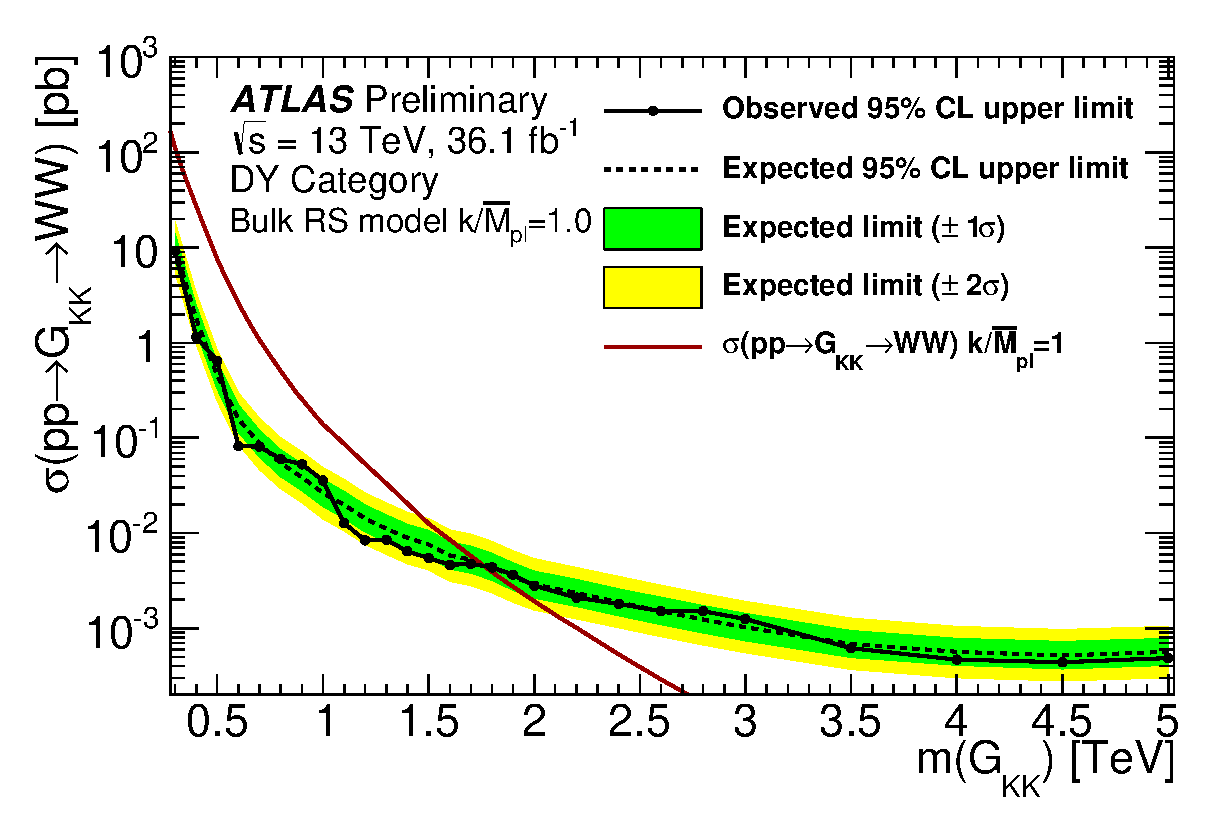
\includegraphics[width=.495\textwidth]{figures/ATLAS-CONF-2017-051_graviton.eps}
  \caption{The observed and expected limits, with 68\% and 95\% uncertainty bands, on the product of the cross-section and branching fraction $\sigma \mathcal{B} (G \rightarrow ZZ)$ for a spin-2 bulk graviton, as a function of the reconstructed mass of the diboson resonance. The coloured lines show the theoretical predictions for $\tilde{k}=1$.~\cite{ATLAS-CONF-2017-051}}
  \label{fig:theory_ATLAS-CONF-2017-051}
\end{figure}

%CMS:\\
%VV all had 2017 B2G-17-001\\%~\cite{bib:CMS-PAS-B2G-17-001}\\
%VH all had 2017 B2G-17-002~\cite{bib:CMS-PAS-B2G-17-002}\\
%VZ 2l 2nu 2017 B2G-16-023~\cite{CMS-PAS-B2G-16-023}\\
%HH 4b 2017 B2G-16-026~\cite{CMS-PAS-B2G-16-026}\\
%VZ 2l 2q 2016 B2G-16-022~\cite{CMS-PAS-B2G-16-022}\\
%VH 2l 2b 2016 B2G-16-003~\cite{Khachatryan:2016cfx}\\
%VW 1l 1nu 2q 2016 B2G-16-020~\cite{CMS-PAS-B2G-16-020}\\
%VZ 2nu 2q B2G-17-005~\cite{CMS-PAS-B2G-17-005}\\
%$WZ, ZZ \rightarrow \ell \bar{\ell} \nu \bar{\nu}$~\cite{CMS-PAS-B2G-16-023}; $HH \rightarrow b\bar{b} b \bar{b}$~\cite{CMS-PAS-B2G-16-026}; SOLO GRAVITONI

%ATLAS:\\
%VV all had 2017 CERN-EP-2017-147~\cite{Aaboud:2017eta}\\
%VH all had 2017 CERN-EP-2017-111~\cite{Aaboud:2017ahz} \\ 
%VW 1l 1nu 2q full 2016 ATLAS-CONF-2017-051~\cite{ATLAS-CONF-2017-051}\\
%VW ICHEP 2016 CERN-EP-2017-146~\cite{ATLAS-CONF-2016-062}\\
%VH lnu 2b ATLAS-CONF-2017-055~\cite{ATLAS-CONF-2017-055}\\
%VZ ICHEP semileptonic  ATLAS-CONF-2016-082~\cite{ATLAS-CONF-2016-082}\\

%{\colour{red} \bf discussion on k/MPL less 1 postponed}\\
%{\colour{red} \bf zero-mode of graviton in the planck brane -- KK graviton in the TeV brane}\\
%{\colour{red} \bf volume suppression vs yukawa suppression}\\

\clearpage

